\documentclass[12pt, a4paper]{article}

\usepackage[utf8]{inputenc}
\usepackage[T1]{fontenc}
\usepackage[provide=*,german]{babel}
\usepackage{csquotes}
% microtype disabled for compatibility
\usepackage{geometry}
\geometry{a4paper, margin=2.5cm}
\usepackage{fancyhdr}
\usepackage{titlesec}
\usepackage{amsmath, amssymb, amsthm}
\usepackage{graphicx}
\usepackage{xcolor}
\usepackage{booktabs}
\usepackage{longtable}
\usepackage{enumitem}
\usepackage{listings}
\usepackage{microtype}
\usepackage{tcolorbox}
\tcbuselibrary{skins, breakable, theorems}
\usepackage{mdframed}
\usepackage{tikz}
\usetikzlibrary{shapes.geometric, arrows.meta, fit, positioning, calc, patterns, decorations.pathmorphing}
\usepackage{pgfplots}
\pgfplotsset{compat=1.18}
\usepackage{subcaption}
\usepackage{hyperref}
\hypersetup{
  colorlinks=true,
  linkcolor=blue!60!black,
  urlcolor=blue!70!black,
  citecolor=green!50!black,
  pdftitle={Zur Verfügung stellen von Dateien in mobilen Betriebssystemen},
  pdfauthor={Stephan Epp},
  pdfsubject={Mobile Computing, Dateiarchitektur, Systemintegration},
}
\usepackage{cleveref}

%------- Farben -------
\definecolor{primblue}{RGB}{25, 60, 140}
\definecolor{secblue}{RGB}{60, 110, 200}
\definecolor{accentgold}{RGB}{200, 160, 20}
\definecolor{lightgray}{RGB}{240, 240, 240}
\definecolor{darkgray}{RGB}{60, 60, 60}
\definecolor{alertred}{RGB}{180, 30, 30}
\definecolor{okgreen}{RGB}{20, 120, 50}
\definecolor{warnorange}{RGB}{210, 100, 0}

%------- Theorem-Umgebungen -------
\newtheorem{definition}{Definition}[section]
\newtheorem{satz}[definition]{Satz}
\newtheorem{lemma}[definition]{Lemma}
\newtheorem{korollar}[definition]{Korollar}
\newtheorem{prinzip}[definition]{Grundsatz}
\newtheorem{konsequenz}[definition]{Konsequenz}
\newtheorem{bemerkung}[definition]{Bemerkung}

%------- tcolorbox-Stile -------
\tcbset{
  grundsatz/.style={
    enhanced, breakable,
    colback=primblue!5,
    colframe=primblue,
    fonttitle=\bfseries,
    title={Grundsatz},
    attach boxed title to top left={xshift=5mm, yshift=-3mm},
    boxed title style={colback=primblue, colframe=primblue!80!black},
    drop shadow,
  },
  warnung/.style={
    enhanced, breakable,
    colback=alertred!5,
    colframe=alertred,
    fonttitle=\bfseries\color{white},
    title={Warnung},
    attach boxed title to top left={xshift=5mm, yshift=-3mm},
    boxed title style={colback=alertred, colframe=alertred!80!black},
  },
  beispiel/.style={
    enhanced, breakable,
    colback=okgreen!5,
    colframe=okgreen!70!black,
    fonttitle=\bfseries,
    title={Beispiel},
    attach boxed title to top left={xshift=5mm, yshift=-3mm},
    boxed title style={colback=okgreen!80!black},
  },
  hinweis/.style={
    enhanced, breakable,
    colback=accentgold!8,
    colframe=accentgold!80!black,
    fonttitle=\bfseries,
    title={Hinweis},
    attach boxed title to top left={xshift=5mm, yshift=-3mm},
    boxed title style={colback=accentgold!90!black},
  },
}

%------- Listings -------
\lstdefinestyle{android}{
  language=Java,
  basicstyle=\ttfamily\footnotesize,
  keywordstyle=\color{primblue}\bfseries,
  commentstyle=\color{okgreen!70!black}\itshape,
  stringstyle=\color{alertred!80!black},
  numberstyle=\tiny\color{darkgray},
  numbers=left, numbersep=8pt,
  backgroundcolor=\color{lightgray},
  frame=single, framerule=0.4pt, rulecolor=\color{darkgray},
  breaklines=true, captionpos=b,
  tabsize=4, showstringspaces=false,
}
\lstdefinestyle{xml}{
  language=XML,
  basicstyle=\ttfamily\footnotesize,
  keywordstyle=\color{secblue}\bfseries,
  commentstyle=\color{darkgray}\itshape,
  stringstyle=\color{alertred!80!black},
  numberstyle=\tiny\color{darkgray},
  numbers=left, numbersep=8pt,
  backgroundcolor=\color{lightgray!60},
  frame=single, rulecolor=\color{darkgray!60},
  breaklines=true, captionpos=b,
}

\title{\textbf{Zur Verfügung stellen von Dateien\\ in mobilen Betriebssystemen}}
\author{Stephan Epp}
\date{25. März 2026}

%============================================================
\begin{document}
%============================================================

\maketitle
\tableofcontents
\newpage

%============================================================
\section{Einleitung und Motivation}
\label{sec:einleitung}
%============================================================

Mobile Betriebssysteme — allen voran Android und iOS — haben im vergangenen Jahrzehnt
eine Architektur herausgebildet, die den Umgang mit Dateien fundamental von klassischen
Desktop-Paradigmen unterscheidet. Während auf traditionellen Computersystemen eine
Datei im Dateisystem des Betriebssystems als primärer Speicherort für persistente Daten
gilt und Anwendungen lediglich lesen und schreiben, wurden auf mobilen Plattformen
gezielt Sandboxing-Mechanismen eingeführt, die jede Anwendung in einem isolierten
Speicherbereich kapseln. Diese Isolierung dient primär der Sicherheit und dem Datenschutz,
erzeugt jedoch zugleich ein strukturelles Spannungsverhältnis: Anwendungen, die Dateien
produzieren — Kameras, Dokumenteneditoren, Audio-Recorder, Mediaplayer — müssen
entscheiden, \emph{wo} diese Dateien residieren und \emph{wer} auf sie zugreifen kann.

In der Praxis hat sich ein klares und ethisch wie technisch gebotenes Prinzip herausgestellt:

\noindent\textbf{Das Bereitstellungsprinzip:} Eine dateiproduzierende mobile Anwendung hat die
erzeugten Dateien dem systemweiten Dateiverwaltungssystem des Betriebssystems
\emph{zur Verfügung zu stellen}. Dateien dürfen nicht dauerhaft im App-eigenen,
für andere Anwendungen und den Benutzer unzugänglichen Speicher verbleiben.

Dieses Prinzip bildet den Kern der vorliegenden Arbeit. Es wird zunächst die technische
Architektur mobiler Betriebssysteme untersucht (\cref{sec:architektur}), dann das
Bereitstellungsprinzip formal definiert und hergeleitet (\cref{sec:prinzip}), anschließend
an konkreten Anwendungsklassen exemplifiziert (\cref{sec:anwendungsklassen}), und
schließlich werden alle Randgebiete und Konsequenzen umfassend diskutiert
(\cref{sec:konsequenzen}).

\subsection{Definitionen}

Der Begriff \enquote{Freigabe} entstammt dem Sprachgebrauch der Praxis und ist historisch
durch die Erfahrung im Umgang mit mobilen Apps entstanden. Er ist berechtigt, weil er
das subjektive Erleben des Benutzers akkurat beschreibt: Eine Datei, die aus einer App
heraus \enquote{freigegeben} wird, ist plötzlich systemweit zugänglich. Dennoch ist
er aus technischer Perspektive ungenau, da er eine vorherige Sperrung impliziert, die
in der korrekten Implementierung gar nicht erst existieren sollte.

\begin{definition}[Zur-Verfügung-Stellen]
\label{def:verfuegbarstellen}
Das \emph{Zur-Verfügung-Stellen} einer Datei bezeichnet den Prozess, durch den eine
dateiproduzierende Anwendung eine erzeugte Datei in einem für das Betriebssystem
und autorisierte Drittanwendungen zugänglichen Speicherbereich ablegt und diesen
Vorgang dem Medienspeicher-System des Betriebssystems signalisiert.
\end{definition}

\begin{bemerkung}
Die Terminologie \enquote{zur Verfügung stellen} ist \enquote{Freigabe} vorzuziehen,
da sie keine nachträgliche Handlung impliziert, sondern den Normalzustand beschreibt:
Eine Datei, die ein Produktionsprozess erzeugt, ist \emph{von Natur aus} dem System
zur Verfügung zu stellen. Dieses Dokument verwendet beide Begriffe äquivalent,
bevorzugt jedoch die präzisere Formulierung.
\end{bemerkung}

%============================================================
\section{Technische Architektur mobiler Betriebssysteme}
\label{sec:architektur}
%============================================================

\subsection{Das Sandboxing-Modell}

Moderne mobile Betriebssysteme basieren auf dem Prinzip der \emph{Anwendungsisolation}.
Jede installierte App erhält einen eigenen, abgeschotteten Speicherbereich, auf den
ausschließlich diese App zugreifen kann. Dieses Modell, bekannt als \emph{Sandboxing},
hat zwei wesentliche Ausprägungen:

\begin{enumerate}[label=\textbf{\arabic*.}]
  \item \textbf{App-privater Speicher (Internal Storage):} Verzeichnisse wie
    \texttt{/data/data/\newline <package>} (Android) oder \texttt{Documents/} (iOS-App-Container),
    auf die ausschließlich die eigene App zugreifen kann.
  \item \textbf{Geteilter / systemweiter Speicher (Shared Storage):} Bereiche wie
    Galerien, Download-Ordner, Musikbibliotheken — zugänglich für Betriebssystem,
    Datei-Manager und anderen autorisierten Apps.
\end{enumerate}

\begin{figure}[ht]
\centering
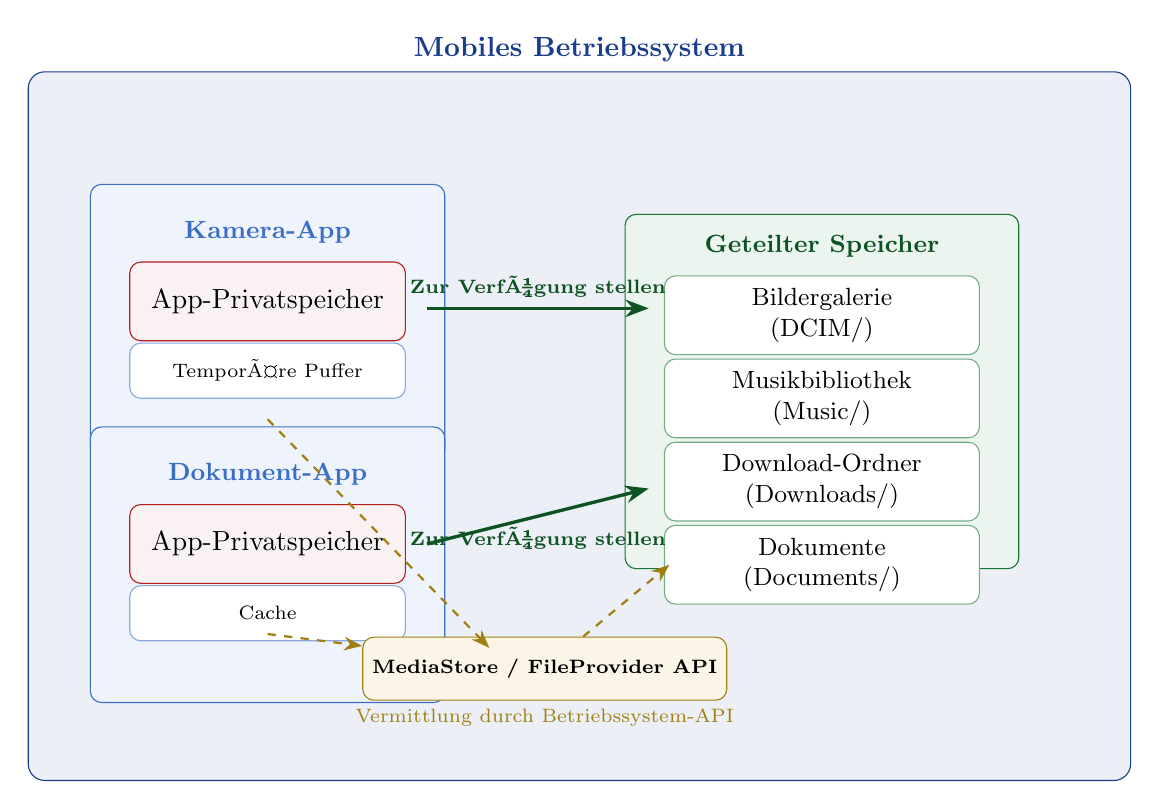
\begin{tikzpicture}[
  box/.style={draw, rounded corners=4pt, minimum width=3.5cm, minimum height=1cm,
              align=center, font=\small},
  arrow/.style={-Stealth, thick},
  sysbox/.style={draw=primblue, fill=primblue!8, rounded corners=6pt},
  appbox/.style={draw=secblue, fill=secblue!8, rounded corners=4pt},
  privbox/.style={draw=alertred, fill=alertred!6, rounded corners=4pt},
  pubbox/.style={draw=okgreen, fill=okgreen!8, rounded corners=4pt},
  scale=0.88
]

% Betriebssystem-Rahmen
\node[sysbox, minimum width=14cm, minimum height=9cm, label={[primblue, font=\bfseries]above:Mobiles Betriebssystem}] (os) at (0,0) {};

% Shared Storage
\node[pubbox, minimum width=5cm, minimum height=4.5cm] (shared) at (3.5, 0.5) {};
\node[font=\bfseries\small, color=okgreen!70!black] at (3.5, 2.6) {Geteilter Speicher};
\node[box, draw=okgreen!60, fill=white, minimum width=4cm] at (3.5, 1.6) {Bildergalerie\\(DCIM/)};
\node[box, draw=okgreen!60, fill=white, minimum width=4cm] at (3.5, 0.4) {Musikbibliothek\\(Music/)};
\node[box, draw=okgreen!60, fill=white, minimum width=4cm] at (3.5, -0.8) {Download-Ordner\\(Downloads/)};
\node[box, draw=okgreen!60, fill=white, minimum width=4cm] at (3.5, -2.0) {Dokumente\\(Documents/)};

% App-Sandbox 1 (Kamera)
\node[appbox, minimum width=4.5cm, minimum height=3.5cm] (app1) at (-4.5, 1.5) {};
\node[font=\bfseries\small, color=secblue] at (-4.5, 2.8) {Kamera-App};
\node[privbox, minimum width=3.5cm, minimum height=1cm] at (-4.5, 1.8) {App-Privatspeicher};
\node[box, draw=secblue!60, fill=white, minimum width=3.5cm, minimum height=0.7cm, font=\scriptsize] at (-4.5, 0.8) {Temporäre Puffer};

% App-Sandbox 2 (Dokument)
\node[appbox, minimum width=4.5cm, minimum height=3.5cm] (app2) at (-4.5, -2) {};
\node[font=\bfseries\small, color=secblue] at (-4.5, -0.7) {Dokument-App};
\node[privbox, minimum width=3.5cm, minimum height=1cm] at (-4.5, -1.7) {App-Privatspeicher};
\node[box, draw=secblue!60, fill=white, minimum width=3.5cm, minimum height=0.7cm, font=\scriptsize] at (-4.5, -2.7) {Cache};

% Arrows: Kamera -> Shared
\draw[arrow, color=okgreen!70!black, very thick] (-2.2, 1.7) -- (1.0, 1.7) 
  node[midway, above, font=\scriptsize\bfseries, color=okgreen!70!black] {Zur Verfügung stellen};

% Arrows: Dokument -> Shared
\draw[arrow, color=okgreen!70!black, very thick] (-2.2, -1.7) -- (1.0, -0.9)
  node[midway, below, font=\scriptsize\bfseries, color=okgreen!70!black] {Zur Verfügung stellen};

% MediaStore
\node[box, draw=accentgold!80!black, fill=accentgold!10, minimum width=3cm, minimum height=0.8cm, font=\scriptsize\bfseries] (ms) at (-0.5, -3.5) {MediaStore / FileProvider API};

\draw[arrow, dashed, color=accentgold!80!black] (ms) -- (1.3, -2.0);
\draw[arrow, dashed, color=accentgold!80!black] (-4.5, -3.0) -- (ms);
\draw[arrow, dashed, color=accentgold!80!black] (-4.5, 0.1) -- (-1.3, -3.2);

\node[font=\scriptsize, color=accentgold!80!black] at (-0.5, -4.2) {Vermittlung durch Betriebssystem-API};

\end{tikzpicture}
\caption{Schematische Darstellung der Speicherarchitektur eines mobilen Betriebssystems.
App-private Bereiche (rot) sind von außen nicht zugänglich; der geteilte Speicher (grün)
ist systemweit verfügbar. Das Zur-Verfügung-Stellen (grüne Pfeile) ist der zentrale Vorgang.}
\label{fig:speicherarchitektur}
\end{figure}

\subsection{Android: Speicherbereiche im Detail}

Unter Android gliedert sich der Speicher seit API-Level 29 (Android 10) durch
\emph{Scoped Storage} in klar definierte Bereiche:

\begin{longtable}{@{}p{3.5cm} p{3.5cm} p{4.5cm} p{2cm}@{}}
\toprule
\textbf{Bereich} & \textbf{Pfad (typisch)} & \textbf{Zugänglichkeit} & \textbf{App-spezifisch} \\
\midrule
\endhead
Internal Storage & \texttt{/data/data/pkg/} & Nur eigene App & Ja \\
External App-Dir & \texttt{/sdcard/Android/data/} & Nur eigene App + Root & Ja \\
Shared DCIM & \texttt{/sdcard/DCIM/} & Alle Apps mit Berechtigung & Nein \\
Shared Music & \texttt{/sdcard/Music/} & Alle Apps mit Berechtigung & Nein \\
Shared Downloads & \texttt{/sdcard/Download/} & Alle Apps mit Berechtigung & Nein \\
Shared Documents & \texttt{/sdcard/Documents/} & Alle Apps mit Berechtigung & Nein \\
\bottomrule
\caption{Speicherbereiche unter Android mit Zugänglichkeit}
\label{tab:android-speicher}
\end{longtable}

\subsection{iOS: Das App-Container-Modell}

Unter iOS existiert ein ähnliches, wenngleich anders benanntes System. Jede App besitzt
einen \emph{App-Container}, der folgende Unterverzeichnisse enthält: \texttt{Documents/}
(app-privat, im iCloud-Backup), \texttt{Library/} (Konfigurationen), \texttt{tmp/}
(temporär). Systemweite Zugänglichkeit wird über das \emph{Files-App-Framework} und
die \emph{Photos Library API} realisiert. Eine dateiproduzierende App muss auf iOS
explizit Dateien über diese APIs dem System zur Verfügung stellen.

\subsection{Die Rolle des MediaStore (Android)}

Der \texttt{MediaStore} ist die zentrale Datenbank unter Android, die alle medienrelevanten
Dateien (Bilder, Videos, Audio, Dokumente) katalogisiert. Er fungiert als Vermittler
zwischen datenproduzierenden Apps und dem Rest des Systems:

\begin{lstlisting}[style=android, caption={Korrekte Uebergabe eines Bildes an den MediaStore unter Android}]
// Korrekte Implementierung: Bild wird dem System zur Verfuegung gestellt
ContentValues values = new ContentValues();
values.put(MediaStore.Images.Media.DISPLAY_NAME, "foto_2026.jpg");
values.put(MediaStore.Images.Media.MIME_TYPE, "image/jpeg");
values.put(MediaStore.Images.Media.RELATIVE_PATH,
           Environment.DIRECTORY_PICTURES + "/MeineApp");

Uri imageUri = getContentResolver().insert(
    MediaStore.Images.Media.EXTERNAL_CONTENT_URI, values);

// Datei in den systemweiten Speicher schreiben
try (OutputStream out = getContentResolver().openOutputStream(imageUri)) {
    bitmap.compress(Bitmap.CompressFormat.JPEG, 95, out);
} // Datei ist nun systemweit zugaenglich -- kein Scan noetig
\end{lstlisting}

%============================================================
\section{Das Bereitstellungsprinzip — Formale Herleitung}
\label{sec:prinzip}
%============================================================

\subsection{Grundlegende Definitionen}

\begin{definition}[Dateiproduzierende Anwendung]
\label{def:dpapp}
Eine \emph{dateiproduzierende Anwendung} $A$ ist eine mobile Softwareanwendung, deren
primärer Zweck oder ein wesentlicher Teilzweck darin besteht, persistente digitale
Dateien zu erzeugen. Formal: $A$ ist dateiproduierend, wenn $\exists\, t: \text{Output}(A, t) \cap \mathcal{F} \neq \emptyset$,
wobei $\mathcal{F}$ die Menge aller möglichen Dateitypen bezeichnet und $t$ einen
Ausführungszeitpunkt darstellt.
\end{definition}

\begin{definition}[App-privater Speicher]
\label{def:privatspeicher}
Der \emph{App-private Speicher} $S_{\text{priv}}(A)$ einer Anwendung $A$ ist der
Speicherbereich, auf den ausschließlich $A$ selbst (und privilegierte Systemprozesse)
lesend und schreibend zugreifen können. Es gilt:
\[
  \forall B \neq A: \text{Access}(B, S_{\text{priv}}(A)) = \bot
\]
\end{definition}

\begin{definition}[Systemweiter Speicher]
\label{def:systemspeicher}
Der \emph{systemweite Speicher} $S_{\text{sys}}$ ist der Speicherbereich, auf den das
Betriebssystem, autorisierte Drittanwendungen und der Benutzer über
Systemwerkzeuge zugreifen können:
\[
  \forall B \in \mathcal{A}_{\text{auth}}: \text{Access}(B, S_{\text{sys}}) = \top
\]
wobei $\mathcal{A}_{\text{auth}}$ die Menge der berechtigten Anwendungen ist.
\end{definition}

\begin{definition}[Bereitstellungsoperation]
\label{def:bereitstellung}
Die \emph{Bereitstellungsoperation} $\Phi: \mathcal{F} \times S_{\text{priv}} \to S_{\text{sys}}$
ist die Abbildung, die eine Datei $f \in \mathcal{F}$ aus dem App-privaten in den
systemweiten Speicher überführt und den Systemmedienspeicher über die neue Datei
informiert:
\[
  \Phi(f) := \big( \text{Move}(f, S_{\text{sys}}),\; \text{Notify}(\text{MediaStore}, f) \big)
\]
\end{definition}

\subsection{Das Bereitstellungsprinzip als formaler Grundsatz}

\begin{prinzip}[Das Bereitstellungsprinzip]
\label{prinzip:bereitstellung}
Sei $A$ eine dateiproduzierende Anwendung und $f \in \mathcal{F}$ eine von $A$ erzeugte
Datei. Dann gilt unter allen Umständen:
\[
  \text{Persist}(f) \Rightarrow \Phi(f)
\]
Das heißt: Jede Datei, die persistent gespeichert werden soll, \textbf{muss} durch die
Bereitstellungsoperation $\Phi$ in den systemweiten Speicher überführt werden.
Die dauerhafte Ablage in $S_{\text{priv}}(A)$ ist unzulässig.
\end{prinzip}

\begin{prinzip}[Verletzungsfall]
\label{prinzip:verletzung}
Eine Anwendung $A$ verletzt das Bereitstellungsprinzip, wenn:
\[
  \exists\, f \in \mathcal{F}: \text{Persist}(f) \wedge \neg\Phi(f) \wedge f \in S_{\text{priv}}(A)
\]
Dies stellt einen schwerwiegenden Implementierungsfehler dar, der Benutzerrechte,
Datensouveränität und Systemintegrität verletzt.
\end{prinzip}

\subsection{Herleitung aus dem Benutzersouveränitätsprinzip}

Das Bereitstellungsprinzip folgt unmittelbar aus dem übergeordneten
\emph{Benutzersouveränitätsprinzip}, das besagt: Der Benutzer eines mobilen Geräts
ist der rechtmäßige Eigentümer aller auf seinem Gerät erzeugten Daten. Daraus folgt:

\begin{satz}[Datensouveränität impliziert Bereitstellungspflicht]
\label{satz:datensouveraenitaet}
Sei $u$ der Benutzer eines mobilen Geräts $D$ und $A$ eine dateiproduzierende
Anwendung auf $D$. Dann gilt:
\[
  \text{Souverän}(u, D) \Rightarrow \text{Zugriffsrecht}(u, f) \quad \forall\, f \in \text{Erzeugt}(A)
\]
Da $\text{Zugriffsrecht}(u, f)$ nur dann erfüllt ist, wenn $f \in S_{\text{sys}}$, folgt
das Bereitstellungsprinzip (\cref{prinzip:bereitstellung}) als notwendige Bedingung.
\end{satz}

\begin{proof}
Der Benutzer $u$ kann auf $S_{\text{priv}}(A)$ ohne spezielle (und üblicherweise nicht
vorhandene) Berechtigungen nicht zugreifen. Folglich ist $\text{Zugriffsrecht}(u, f) = \bot$
für $f \in S_{\text{priv}}(A)$. Dies steht im Widerspruch zu $\text{Souverän}(u, D)$.
Daher muss $f \in S_{\text{sys}}$ gelten.
\end{proof}

%============================================================
\section{Anwendungsklassen und ihre Bereitstellungspflicht}
\label{sec:anwendungsklassen}
%============================================================

\subsection{Die Kamera-Applikation}

Die Kamera-Applikation ist das paradigmatische Beispiel einer dateiproduzierenden App.
Ihre Ausgabe — fotografische Bilder und Videoaufnahmen — sind Primärdaten, die unmittelbar
nach ihrer Erzeugung dem System zur Verfügung gestellt werden müssen.

\subsubsection{Korrekte Implementierung unter Android}

\begin{lstlisting}[style=android, caption={Kamerabild korrekt an MediaStore uebergeben}]
public void saveImageToGallery(Bitmap bitmap, Context context) {
    ContentValues values = new ContentValues();
    values.put(MediaStore.Images.Media.DISPLAY_NAME,
               "IMG_" + System.currentTimeMillis() + ".jpg");
    values.put(MediaStore.Images.Media.MIME_TYPE, "image/jpeg");
    values.put(MediaStore.Images.Media.DATE_ADDED,
               System.currentTimeMillis() / 1000);
    values.put(MediaStore.Images.Media.RELATIVE_PATH,
               Environment.DIRECTORY_DCIM + "/Camera");
    values.put(MediaStore.Images.Media.IS_PENDING, 1); // Schreibe-Lock

    Uri uri = context.getContentResolver().insert(
        MediaStore.Images.Media.EXTERNAL_CONTENT_URI, values);

    try (OutputStream out = context.getContentResolver()
                                   .openOutputStream(uri)) {
        bitmap.compress(Bitmap.CompressFormat.JPEG, 95, out);
        // Schreibe-Lock aufheben: Datei jetzt systemweit sichtbar
        values.clear();
        values.put(MediaStore.Images.Media.IS_PENDING, 0);
        context.getContentResolver().update(uri, values, null, null);
    } catch (IOException e) {
        context.getContentResolver().delete(uri, null, null);
        throw new RuntimeException("Fehler beim Speichern", e);
    }
}
\end{lstlisting}

\subsubsection{Verletzungsfall: Privatspeicherung}

\noindent\textbf{Anti-Pattern: Datei im App-Privatspeicher.}\par
Die folgende Implementierung \textbf{verletzt} das Bereitstellungsprinzip:
\begin{lstlisting}[style=android, numbers=none]
// FALSCH: Bild wird im App-privaten Verzeichnis gespeichert
File privateDir = context.getFilesDir(); // App-privat!
File imageFile = new File(privateDir, "foto.jpg");
// Kein MediaStore-Eintrag, keine systemweite Sichtbarkeit
// Benutzer kann Datei nicht in Galerie sehen
// Datei geht bei App-Deinstallation verloren
\end{lstlisting}

\subsection{Dokumenteneditoren}

Textverarbeitungsprogramme, Tabellenkalkulatoren, PDF-Editoren und verwandte
Anwendungstypen produzieren Dokumente, die in der Regel langfristig gespeichert und
von anderen Anwendungen weiterverarbeitet werden sollen.

\noindent\textbf{Beispiel — Dokumenten-App unter Android.}\par
Eine Dokumenten-App, die eine PDF-Datei erzeugt, muss diese in
\texttt{/sdcard/Documents/} (über \texttt{MediaStore.Files} oder Storage Access Framework)
ablegen und den entsprechenden MIME-Typ \texttt{application/pdf} registrieren.
Die Datei ist dann über jeden installierten Dateimanager und jede PDF-Leseanwendung
zugänglich.

\subsubsection{Storage Access Framework (SAF)}

Unter Android bietet das \emph{Storage Access Framework} einen standardisierten
Mechanismus, um Dateien systemweit zur Verfügung zu stellen, ohne direkte
Dateipfad-Abhängigkeiten zu erzeugen:

\begin{lstlisting}[style=android, caption={Dokument ueber SAF systemweit bereitstellen}]
// Benutzer waehlt Speicherort (systemweiter Dialog)
Intent intent = new Intent(Intent.ACTION_CREATE_DOCUMENT);
intent.addCategory(Intent.CATEGORY_OPENABLE);
intent.setType("application/pdf");
intent.putExtra(Intent.EXTRA_TITLE, "bericht_2026.pdf");
startActivityForResult(intent, REQUEST_CODE_CREATE_DOC);

// Im Callback: Datei in den vom Benutzer gewaehlten Pfad schreiben
@Override
protected void onActivityResult(int requestCode, int result, Intent data) {
    if (requestCode == REQUEST_CODE_CREATE_DOC
        && result == RESULT_OK) {
        Uri uri = data.getData(); // Systemweiter URI
        try (OutputStream out = getContentResolver()
                                    .openOutputStream(uri)) {
            writePdfContent(out); // Dokument schreiben
            // Datei ist nun systemweit verfuegbar
        }
    }
}
\end{lstlisting}

\subsection{Audio-Anwendungen: Recorder und Downloader}

\subsubsection{Audio-Recorder}

Aufnahme-Anwendungen erzeugen Audiodateien (WAV, MP3, AAC, FLAC). Diese müssen
nach Abschluss der Aufnahme in der Musikbibliothek oder dem Download-Ordner des
Systems registriert werden:

\begin{lstlisting}[style=android, caption={Audioaufnahme dem System bereitstellen}]
ContentValues values = new ContentValues();
values.put(MediaStore.Audio.Media.DISPLAY_NAME, "aufnahme.m4a");
values.put(MediaStore.Audio.Media.MIME_TYPE, "audio/mp4");
values.put(MediaStore.Audio.Media.RELATIVE_PATH,
           Environment.DIRECTORY_MUSIC + "/Aufnahmen");
values.put(MediaStore.Audio.Media.IS_MUSIC, 1);

Uri audioUri = getContentResolver().insert(
    MediaStore.Audio.Media.EXTERNAL_CONTENT_URI, values);
// Audiodatei schreiben und IS_PENDING auf 0 setzen
\end{lstlisting}

\subsubsection{MP3-Downloader}

Anwendungen, die Audiodateien aus dem Internet herunterladen, stellen einen wichtigen
Grenzfall dar. Der Download-Prozess erzeugt eine Datei, die dem Benutzer dauerhaft
zur Verfügung stehen soll:

\begin{enumerate}[label=\textbf{\arabic*:}]
  \item \textbf{Download initiieren:} Die Datei wird temporär in einen Arbeitsspeicher
    geladen.
  \item \textbf{Überprüfung:} Integrität und Lizenzstatus der Datei werden geprüft.
  \item \textbf{Bereitstellung:} Die abgeschlossene Datei wird über \texttt{MediaStore}
    oder \texttt{DownloadMana-\newline ger} in den systemweiten Speicher (\texttt{Downloads/}
    oder \texttt{Music/}) überführt.
  \item \textbf{Benachrichtigung:} Das Betriebssystem wird über die neue Datei
    informiert.
\end{enumerate}

\begin{lstlisting}[style=android, caption={Systemkonformer Datei-Download per DownloadManager}]
DownloadManager.Request request = new DownloadManager.Request(
    Uri.parse("https://example.com/audio.mp3"))
    .setTitle("Audiodatei")
    .setDescription("Download laeuft...")
    .setNotificationVisibility(
        DownloadManager.Request.VISIBILITY_VISIBLE_NOTIFY_COMPLETED)
    .setDestinationInExternalPublicDir(
        Environment.DIRECTORY_MUSIC, "audiodatei.mp3") // Systemweit!
    .setMimeType("audio/mpeg");

DownloadManager dm = (DownloadManager) getSystemService(DOWNLOAD_SERVICE);
long downloadId = dm.enqueue(request);
// Datei wird automatisch im systemweiten Music/-Ordner gespeichert
\end{lstlisting}

\subsection{Videobearbeitungsanwendungen}

Videobearbeitungs-Apps exportieren fertige Videos in den systemweiten
Medienspeicher. Zwischendateien (Schnittdaten, Projekte, Render-Cache) können
im App-privaten Speicher verbleiben — das fertige Exportprodukt jedoch
\emph{muss} systemweit bereitgestellt werden.

\subsection{QR-Code- und Barcode-Generatoren}

Anwendungen, die Bilder (QR-Codes, Barcodes) erzeugen, müssen diese auf Wunsch
des Benutzers in die Galerie speichern — nicht nur im App-internen Cache.

\subsection{Zusammenfassung der Anwendungsklassen}

\begin{figure}[ht]
\centering
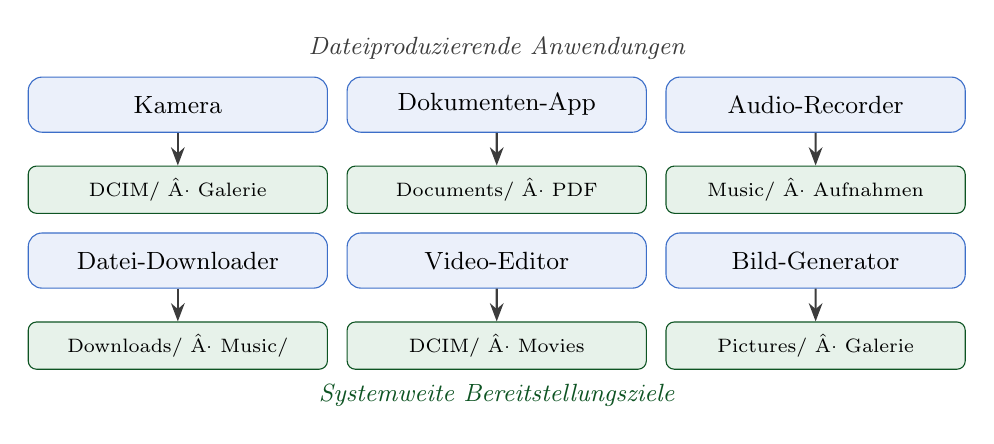
\begin{tikzpicture}[
  node distance=0.6cm,
  appclass/.style={draw=secblue, fill=secblue!10, rounded corners=5pt, 
                   minimum width=3.8cm, minimum height=0.7cm, font=\small, align=center},
  output/.style={draw=okgreen!70!black, fill=okgreen!10, rounded corners=3pt,
                 minimum width=3.8cm, minimum height=0.6cm, font=\scriptsize},
  arrow/.style={-Stealth, thick, color=darkgray},
  scale=0.9
]

\node[appclass] (cam)  at (0, 0)    {Kamera};
\node[appclass] (doc)  at (4.5, 0)  {Dokumenten-App};
\node[appclass] (aud)  at (9, 0)    {Audio-Recorder};
\node[appclass] (dl)   at (0, -2.2) {Datei-Downloader};
\node[appclass] (vid)  at (4.5, -2.2) {Video-Editor};
\node[appclass] (qr)   at (9, -2.2)  {Bild-Generator};

\node[output] (dcim)  at (0, -1.2)   {DCIM/ · Galerie};
\node[output] (docs)  at (4.5, -1.2) {Documents/ · PDF};
\node[output] (music) at (9, -1.2)   {Music/ · Aufnahmen};
\node[output] (down)  at (0, -3.4)   {Downloads/ · Music/};
\node[output] (vidout)at (4.5, -3.4) {DCIM/ · Movies};
\node[output] (pics)  at (9, -3.4)   {Pictures/ · Galerie};

\draw[arrow] (cam) -- (dcim);
\draw[arrow] (doc) -- (docs);
\draw[arrow] (aud) -- (music);
\draw[arrow] (dl)  -- (down);
\draw[arrow] (vid) -- (vidout);
\draw[arrow] (qr)  -- (pics);

% Label
\node[color=darkgray, font=\small\itshape] at (4.5, 0.8) {Dateiproduzierende Anwendungen};
\node[color=okgreen!70!black, font=\small\itshape] at (4.5, -4.1) {Systemweite Bereitstellungsziele};

\end{tikzpicture}
\caption{Ãœbersicht der Anwendungsklassen und ihrer jeweiligen Bereitstellungsziele im systemweiten Speicher.}
\label{fig:anwendungsklassen}
\end{figure}

%============================================================
\section{Konsequenzen des Bereitstellungsprinzips}
\label{sec:konsequenzen}
%============================================================

\subsection{Konsequenzen für den Benutzer}

\subsubsection{Datensouveränität und Kontrolle}

Das Bereitstellungsprinzip ist die technische Umsetzung von Datensouveränität.
Wenn eine App Dateien nur im App-privaten Speicher behält, verliert der Benutzer
die effektive Kontrolle über seine eigenen Daten. Dies hat mehrere unmittelbare
Folgen:

\noindent\textbf{Benutzerauswirkungen bei Verletzung des Bereitstellungsprinzips:}
\begin{itemize}[leftmargin=*]
  \item \textbf{Datenverlust bei Deinstallation:} App-private Daten werden bei
    Deinstallation unwiederbringlich gelöscht.
  \item \textbf{Unmöglichkeit des App-Wechsels:} Der Benutzer ist an die
    produzierende App gebunden, da Konkurrenzprodukte nicht auf die Daten
    zugreifen können.
  \item \textbf{Keine Backup-Integration:} Systemseitige Backups erfassen den
    App-privaten Speicher nur eingeschränkt oder gar nicht.
  \item \textbf{Keine Mediensuche:} Dateien sind in der systemweiten Galerie,
    im Dateimanager und in Suchfunktionen nicht auffindbar.
\end{itemize}

\begin{konsequenz}[Benutzerautonomie]
Das Bereitstellungsprinzip ist eine notwendige Bedingung für Benutzerautonomie
auf mobilen Geräten. Seine Verletzung erzeugt eine faktische Abhängigkeit
(\emph{Vendor Lock-in}) auf Dateiebene.
\end{konsequenz}

\subsubsection{Datenpersistenz und Langzeitspeicherung}

Dateien im systemweiten Speicher überleben die deinstallation der erzeugenden App.
Dies ist für den Benutzer grundlegend: Ein Foto bleibt auch dann erhalten, wenn
die Kamera-App deinstalliert oder durch eine andere ersetzt wird.

\begin{figure}[ht]
\centering
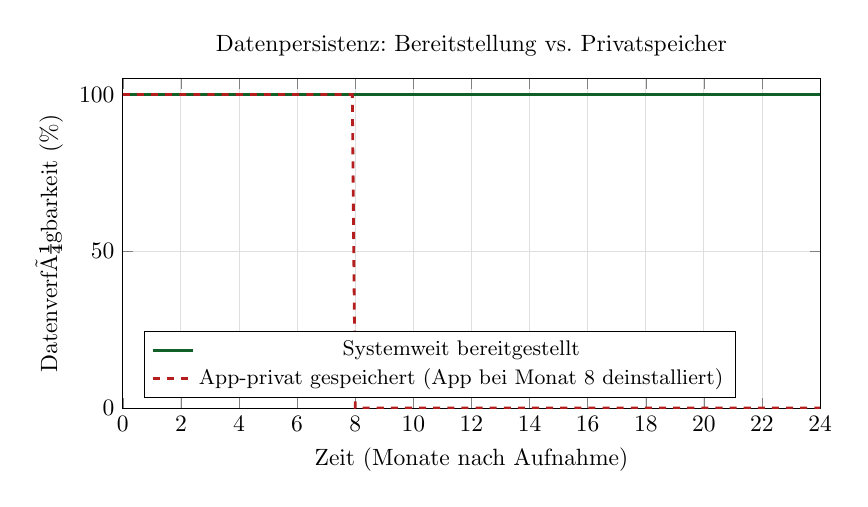
\begin{tikzpicture}[scale=0.85]
  \begin{axis}[
    xlabel={Zeit (Monate nach Aufnahme)},
    ylabel={Datenverfügbarkeit (\%)},
    xmin=0, xmax=24, ymin=0, ymax=105,
    legend pos=south west,
    grid=major, grid style={gray!25},
    title={Datenpersistenz: Bereitstellung vs. Privatspeicher},
    width=12cm, height=6.5cm,
    legend style={font=\small}
  ]
  % Systemweite Datei: stabil auf 100%
  \addplot[color=okgreen!80!black, very thick, mark=none] 
    coordinates {(0,100)(6,100)(12,100)(18,100)(24,100)};
  \addlegendentry{Systemweit bereitgestellt}

  % App-privat: fällt bei Deinstallation auf 0
  \addplot[color=alertred, very thick, mark=none, dashed]
    coordinates {(0,100)(7.9,100)(8,0)(24,0)};
  \addlegendentry{App-privat gespeichert (App bei Monat 8 deinstalliert)}

  % Annotation
  \draw[thick, -Stealth, color=alertred] (9, 15) -- (8.2, 5);
  \node[align=center, font=\scriptsize, color=alertred] at (13, 18) 
    {Deinstallation der App\\→ Datenverlust};
  \end{axis}
\end{tikzpicture}
\caption{Datenpersistenz über die Zeit: Systemweit bereitgestellte Dateien sind dauerhaft
verfügbar; App-privat gespeicherte Dateien gehen bei Deinstallation der App verloren.}
\label{fig:persistenz}
\end{figure}

\subsection{Konsequenzen für die Softwareentwicklung}

\subsubsection{API-Wahl und Architekturentscheidungen}

Entwickler müssen von Beginn an die korrekte API für Dateispeicherung wählen.
Die Wahl des falschen APIs (z.\,B. \texttt{getFilesDir()} statt \texttt{MediaStore}
für persistente Mediendateien) ist ein fundamentaler Architekturmangel, der
nachträglich schwer zu korrigieren ist.

\begin{satz}[API-Äquivalenz]
\label{satz:api}
Für jede Datei $f$ vom Typ $\tau \in \{\text{Bild, Video, Audio, Dokument}\}$
existiert eine eindeutige Ziel-API $\text{API}(\tau)$ im mobilen Betriebssystem,
über die $f$ korrekt dem System zur Verfügung zu stellen ist:
\[
  \text{API}(\tau) = \begin{cases}
    \text{MediaStore.Images} & \text{falls } \tau = \text{Bild} \\
    \text{MediaStore.Video}  & \text{falls } \tau = \text{Video} \\
    \text{MediaStore.Audio}  & \text{falls } \tau = \text{Audio} \\
    \text{MediaStore.Files}  & \text{falls } \tau = \text{Dokument} \\
    \text{DownloadManager}   & \text{falls } \tau = \text{Sonstiges}
  \end{cases}
\]
\end{satz}

\begin{longtable}{@{}p{2.5cm} p{3.5cm} p{3.5cm} p{3cm}@{}}
\toprule
\textbf{Dateityp} & \textbf{Korrekte API (Android)} & \textbf{Korrekte API (iOS)} & \textbf{Zielverzeichnis} \\
\midrule
\endhead
Bild & \texttt{MediaStore.Images} & \texttt{PHPhotoLibrary} & \texttt{DCIM/} \\
Video & \texttt{MediaStore.Video} & \texttt{PHPhotoLibrary} & \texttt{DCIM/} \\
Audio & \texttt{MediaStore.Audio} & \texttt{MPMediaLibrary} & \texttt{Music/} \\
Dokument & \texttt{MediaStore.Files} / SAF & UIDocumentPicker & \texttt{Documents/} \\
Download & \texttt{DownloadManager} & URLSession + FileManager & \texttt{Downloads/} \\
\bottomrule
\caption{Korrekte APIs für verschiedene Dateitypen auf Android und iOS}
\label{tab:apis}
\end{longtable}

\subsubsection{Berechtigungssystem und Datenschutz}

Das korrekte Zur-Verfügung-Stellen erfordert auf modernen Android-Versionen
(API 33+) granulare Berechtigungen:

\begin{lstlisting}[style=xml, caption={AndroidManifest.xml: Korrekte Berechtigungen fuer Medienzugriff}]
<manifest>
    <!-- Schreiben in systemweite Medienbereiche (bis API 28) -->
    <uses-permission android:name=
        "android.permission.WRITE_EXTERNAL_STORAGE"
        android:maxSdkVersion="28" />
    
    <!-- Zugriff auf Bilder (API 33+) -->
    <uses-permission android:name=
        "android.permission.READ_MEDIA_IMAGES" />
    
    <!-- Zugriff auf Videos (API 33+) -->
    <uses-permission android:name=
        "android.permission.READ_MEDIA_VIDEO" />
    
    <!-- Zugriff auf Audio (API 33+) -->
    <uses-permission android:name=
        "android.permission.READ_MEDIA_AUDIO" />
    
    <!-- Kamera-Berechtigung -->
    <uses-permission android:name=
        "android.permission.CAMERA" />
</manifest>
\end{lstlisting}

\subsubsection{FileProvider für App-zu-App-Kommunikation}

Wenn eine dateiproduzierende App eine Datei direkt an eine andere App übergeben
möchte (z.\,B. \enquote{Teilen} einer gerade erstellten Datei), ohne sie zunächst
in den systemweiten Speicher zu schreiben, muss der \texttt{FileProvider}
verwendet werden:

\begin{lstlisting}[style=android, caption={FileProvider fuer temporaere Dateiuebergabe}]
// FileProvider liefert einen Content-URI statt eines Dateipfads
File tempFile = new File(getCacheDir(), "temp_share.pdf");
// Datei erzeugen ...

Uri contentUri = FileProvider.getUriForFile(
    this,
    "de.epp.meinapp.fileprovider",
    tempFile);

Intent shareIntent = new Intent(Intent.ACTION_SEND);
shareIntent.setType("application/pdf");
shareIntent.putExtra(Intent.EXTRA_STREAM, contentUri);
shareIntent.addFlags(Intent.FLAG_GRANT_READ_URI_PERMISSION);
startActivity(Intent.createChooser(shareIntent, "Teilen via"));
\end{lstlisting}

\begin{bemerkung}
FileProvider ist für \emph{temporäre} Übergaben geeignet; für dauerhafte
systemweite Verfügbarkeit muss die Datei dennoch über \texttt{MediaStore}
oder SAF bereitgestellt werden.
\end{bemerkung}

\subsection{Konsequenzen für die Systemintegrität}

\subsubsection{Medienscan und Indexierung}

Das Betriebssystem führt regelmäßige Media-Scans durch, um den \texttt{MediaStore}
aktuell zu halten. Wenn eine App Dateien ohne \texttt{MediaStore}-Eintrag in
(theoretisch zugängliche) Bereiche schreibt, kann es zu Verzögerungen bei der
Sichtbarkeit kommen. Die korrekte Implementierung nutzt \texttt{MediaStore.insert()}
oder \texttt{MediaScannerConnection.scanFile()} unmittelbar nach dem Schreibvorgang.

\begin{lstlisting}[style=android, caption={Expliziter MediaScan (Fallback, Legacy-Code)}]
// Fuer aeltere API-Level ohne automatischen MediaStore-Eintrag
MediaScannerConnection.scanFile(
    context,
    new String[]{ file.getAbsolutePath() },
    new String[]{ "image/jpeg" },
    (path, uri) -> {
        // Scan abgeschlossen: Datei nun im MediaStore sichtbar
        Log.d("MediaScan", "Datei verfuegbar unter: " + uri);
    }
);
\end{lstlisting}

\subsubsection{Speicherbereinigung und Lifecycle}

Das Betriebssystem kann unter Speicherdruck App-private Caches bereinigen,
ohne den Benutzer zu informieren. Dateien im App-privaten \texttt{cacheDir()} sind
\emph{nicht persistent}. Dieser Mechanismus illustriert, warum dauerhafte Dateien
\emph{niemals} im App-privaten Speicher verbleiben dürfen.

\begin{konsequenz}[Systemkohärenz]
Wird das Bereitstellungsprinzip flächendeckend eingehalten, entsteht ein
kohärentes Dateisystem, in dem alle datenproduzierenden Aktivitäten des Benutzers
an einem zentralen, systemweit zugänglichen Ort reflektiert werden. Dies ist
eine Grundvoraussetzung für ein funktionstüchtiges und benutzerfreundliches
Betriebssystem.
\end{konsequenz}

\subsection{Konsequenzen für Sicherheit und Datenschutz}

\subsubsection{Das Paradox der Sandbox}

Ironischerweise kann die Sandboxing-Architektur zu Datenschutzverletzungen
führen, wenn sie missbraucht wird: Eine App, die Dateien \emph{nur} im
App-privaten Speicher behält, entzieht diese Dateien der Kontrolle des
Benutzers, obwohl das Sandboxing eigentlich dessen Schutz dienen soll.

\begin{satz}[Sandbox-Paradox]
Die Sandboxing-Architektur mobiler Betriebssysteme, konzipiert als Schutzmaßnahme
für den Benutzer, kann durch Nicht-Bereitstellung produzierter Dateien zu einer
Einschränkung der Benutzerrechte pervertiert werden. Es gilt:
\[
  \text{Sandbox}(A) + \neg\Phi(f) \Rightarrow \text{EffektiverDateinentzug}(u, f)
\]
\end{satz}

\subsubsection{DSGVO und Datensouveränität}

Im europäischen Rechtsraum ergibt sich eine datenschutzrechtliche Dimension:
Die Daten\-schutz-Grundverordnung (DSGVO) garantiert Betroffenen unter anderem
das Recht auf Datenzugang (Art. 15 DSGVO) und Datenübertragbarkeit (Art. 20 DSGVO).
Eine App, die vom Benutzer produzierte Dateien im App-privaten Speicher einschließt,
erschwert oder verhindert die Wahrnehmung dieser Rechte.

\noindent\textbf{Rechtliche Konsequenz.} Apps, die nutzergenerierte Dateien im App-privaten Speicher einschließen und
dem Benutzer den Zugang zu seinen eigenen Daten systematisch verwehren,
können gegen Art. 15 und Art. 20 DSGVO verstoßen, wenn diese Daten als
personenbezogene Daten zu qualifizieren sind.

\subsubsection{Sicherheit: Zugriffssteuerung durch das Betriebssystem}

Der systemweite Speicher ist \emph{nicht} unkontrolliert zugänglich. Unter
Android müssen Apps seit API 23 Laufzeitberechtigungen für den Medienzugriff
einholen; unter iOS gilt ein vergleichbares Modell. Das Betriebssystem stellt
sicher, dass nur berechtigte Apps auf die Dateien zugreifen können — ein
Sicherheitsgewinn gegenüber unkontrollierter App-privater Hortung.

\subsection{Konsequenzen für Interoperabilität und Ökosystem}

\subsubsection{App-übergreifende Workflows}

Wenn dateiproduzierende Apps das Bereitstellungsprinzip einhalten, ermöglichen
sie komplexe, app-übergreifende Workflows. Beispiele:

\begin{enumerate}[label=\textbf{\arabic*.}]
  \item \textbf{Foto-Workflow:} Kamera-App erzeugt Bild → Galerie zeigt es an →
    Bearbeitungs-App öffnet es → Teilen-Dialog übermittelt es → Cloud-Sync
    sichert es. Jeder dieser Schritte funktioniert nur, wenn das Bild systemweit
    verfügbar ist.
  \item \textbf{Dokument-Workflow:} Dokumenten-App erzeugt PDF → E-Mail-App
    hängt es an → Drucker-App druckt es → Cloud-Speicher synchronisiert es.
  \item \textbf{Audio-Workflow:} Recorder-App nimmt Sprache auf → Transkriptions-App
    verarbeitet die Audiodatei → Texteditor öffnet das Transkript.
\end{enumerate}

\subsubsection{Cloud-Integration und Synchronisierung}

Systemweite Cloud-Sync-Dienste (Google Photos, iCloud, OneDrive) operieren auf
dem systemweiten Dateisystem. Nur bereitgestellte Dateien werden automatisch
synchronisiert und gesichert.

\begin{konsequenz}[Cloud-Sync]
Das Bereitstellungsprinzip ist eine notwendige Bedingung für die automatische
Cloud-Synchronisierung und damit für die Datensicherheit des Benutzers.
\end{konsequenz}

\subsubsection{Barrierefreiheit und Assistivtechnologien}

Assistivtechnologien (Screenreader, Dokumenten-Vorlesedienste, Braille-Ausgabe)
operieren auf systemweit zugänglichen Dateien. Eine App, die Dateien einschließt,
schließt damit auch Benutzer mit Behinderungen von ihren eigenen Inhalten aus —
ein klarer Verstoß gegen Barrierefreiheitsgrundsätze.

\subsection{Konsequenzen für Backup und Gerätewechsel}

\subsubsection{Systemseitiges Backup}

Sowohl Android (Auto Backup) als auch iOS (iCloud Backup) sichern den systemweiten
Speicher vollständig. App-private Daten werden nur bei expliziter Konfiguration
durch den App-Entwickler gesichert — und diese Konfiguration ist fehleranfällig
und nicht standardisiert.

\begin{figure}[ht]
\centering
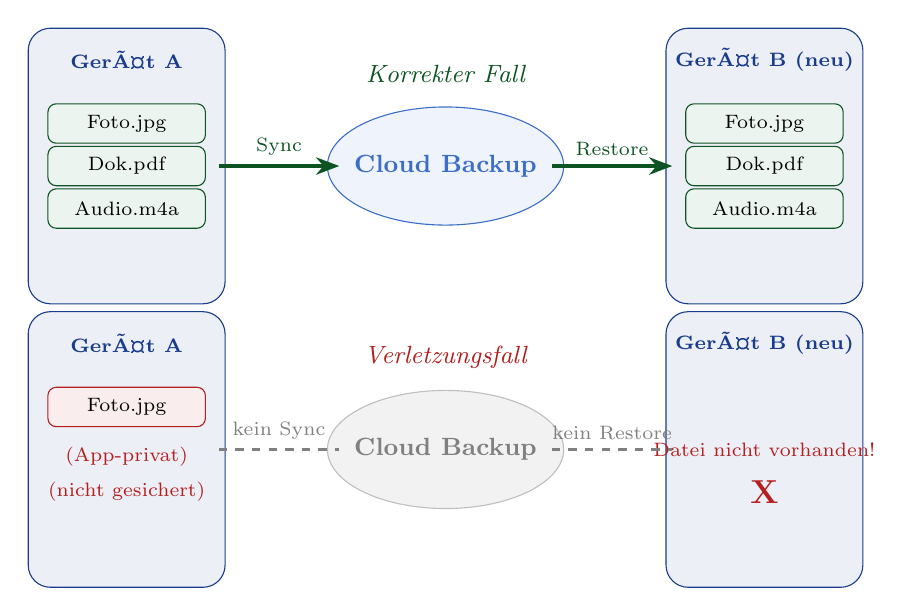
\begin{tikzpicture}[
  node distance=1.2cm,
  device/.style={draw=primblue, fill=primblue!8, rounded corners=8pt,
                 minimum width=2.5cm, minimum height=3.5cm},
  cloud/.style={draw=secblue, fill=secblue!8, ellipse,
                minimum width=3cm, minimum height=1.5cm},
  file/.style={draw=okgreen!70!black, fill=okgreen!8, rounded corners=3pt,
               minimum width=2cm, minimum height=0.5cm, font=\scriptsize},
  arrow/.style={-Stealth, thick},
  scale=0.9
]

\node[device] (d1) at (0, 0) {};
\node[font=\scriptsize\bfseries, color=primblue] at (0, 1.5) {Gerät A};
\node[file] at (0, 0.6) {Foto.jpg};
\node[file] at (0, -0.0) {Dok.pdf};
\node[file] at (0, -0.6) {Audio.m4a};

\node[cloud] (cloud) at (4.5, 0) {};
\node[font=\small\bfseries, color=secblue] at (4.5, 0) {Cloud Backup};

\node[device] (d2) at (9, 0) {};
\node[font=\scriptsize\bfseries, color=primblue] at (9, 1.5) {Gerät B (neu)};
\node[file] at (9, 0.6) {Foto.jpg};
\node[file] at (9, -0.0) {Dok.pdf};
\node[file] at (9, -0.6) {Audio.m4a};

\draw[arrow, color=okgreen!70!black, very thick] (1.3, 0) -- (3.0, 0)
  node[midway, above, font=\scriptsize, color=okgreen!70!black] {Sync};
\draw[arrow, color=okgreen!70!black, very thick] (6.0, 0) -- (7.7, 0)
  node[midway, above, font=\scriptsize, color=okgreen!70!black] {Restore};

% Verletzungsfall darunter
\node[device] (d3) at (0, -4) {};
\node[font=\scriptsize\bfseries, color=primblue] at (0, -2.5) {Gerät A};
\node[draw=alertred, fill=alertred!8, rounded corners=3pt,
      minimum width=2cm, minimum height=0.5cm, font=\scriptsize] at (0, -3.4) {Foto.jpg};
\node[font=\scriptsize, color=alertred] at (0, -4.1) {(App-privat)};
\node[font=\scriptsize, color=alertred] at (0, -4.6) {(nicht gesichert)};

\node[cloud, draw=gray!50, fill=gray!10] (cloud2) at (4.5, -4) {};
\node[font=\small\bfseries, color=gray] at (4.5, -4) {Cloud Backup};

\node[device] (d4) at (9, -4) {};
\node[font=\scriptsize\bfseries, color=primblue] at (9, -2.5) {Gerät B (neu)};
\node[font=\scriptsize, color=alertred] at (9, -4) {Datei nicht vorhanden!};
\node[font=\large, color=alertred] at (9, -4.6) {\textbf{X}};

\draw[dashed, color=gray, thick] (1.3, -4) -- (3.0, -4)
  node[midway, above, font=\scriptsize, color=gray] {kein Sync};
\draw[dashed, color=gray, thick] (6.0, -4) -- (7.7, -4)
  node[midway, above, font=\scriptsize, color=gray] {kein Restore};

\node[font=\small\itshape, color=okgreen!70!black] at (4.5, 1.3) {Korrekter Fall};
\node[font=\small\itshape, color=alertred] at (4.5, -2.7) {Verletzungsfall};

\end{tikzpicture}
\caption{Backup und Gerätewechsel: Korrekt bereitgestellte Dateien werden gesichert und
auf neuen Geräten wiederhergestellt; App-privat gespeicherte Dateien gehen verloren.}
\label{fig:backup}
\end{figure}

\subsubsection{Gerätewechsel und Migration}

Bei einem Gerätewechsel — oder beim Wechsel zwischen Android und iOS über
Migrationswerkzeuge — sind ausschließlich systemweit verfügbare Dateien übertragbar.
App-private Dateien können in der Regel nicht migriert werden, auch nicht durch
Hersteller-Migrationswerkzeuge wie \enquote{Move to iOS} oder \enquote{Google
Backup \& Restore}.

\subsection{Konsequenzen für das App-Ökosystem und den Wettbewerb}

\subsubsection{Gegen Vendor Lock-in auf Dateiebene}

Apps, die das Bereitstellungsprinzip verletzen, erzeugen einen unzulässigen
\emph{Vendor Lock-in}: Der Benutzer ist an die App gebunden, weil seine Daten
in ihr \enquote{gefangen} sind. Dies ist nicht nur ein technisches Problem,
sondern ein wettbewerbspolitisches:

\begin{konsequenz}[Wettbewerbsverzerrung]
Eine App, die Benutzerdaten im App-privaten Speicher einschließt, schafft
künstliche Wechselbarrieren und verstößt gegen den Grundsatz des fairen
Wettbewerbs im App-Ökosystem. Behörden im Bereich des Digitalmarktrechts
(Digital Markets Act, EU) adressieren solche Praktiken zunehmend.
\end{konsequenz}

\subsubsection{Kompatibilität mit App-Store-Richtlinien}

Sowohl der Google Play Store als auch der Apple App Store haben in ihren
Entwicklerrichtlinien Anforderungen formuliert, die implizit oder explizit
das Bereitstellungsprinzip fordern:

\begin{itemize}[leftmargin=*]
  \item Google Play: \emph{User Data Policy} verlangt, dass Apps mit nutzererzeugten
    Daten verantwortungsvoll umgehen.
  \item Apple App Store: \emph{App Store Review Guidelines} (Abschnitt 5.1)
    verlangen, dass Apps den Datenzugang für Benutzer sicherstellen.
\end{itemize}

\subsection{Konsequenzen für Fehlerdiagnose und Debugging}

\subsubsection{Auffindbarkeit von Fehlern}

Wenn Dateien im App-privaten Speicher gespeichert werden, sind sie für
Debugging-Werkzeuge (Android Debug Bridge, Xcode File Inspector) nur mit
erhöhten Berechtigungen (root / dev-Modus) zugänglich. Dies erschwert
die Fehlerdiagnose bei Produktionsproblemen.

\subsubsection{Testbarkeit}

Automationstests, die das Vorhandensein einer Datei nach einer App-Aktion
prüfen, müssen auf den systemweiten Speicher zugreifen können. Bei
korrekter Implementierung sind solche Tests einfach zu schreiben; bei
App-privater Speicherung erfordern sie privilegierten Zugang.

\begin{lstlisting}[style=android, caption={Automatisierter Test: Pruefung der systemweiten Bereitstellung}]
@Test
public void testKamerafoto_wirdInGalerieBereitgestellt() {
    // Foto aufnehmen
    instrumentation.performCamera();
    
    // Pruefen ob Datei im MediaStore vorhanden (systemweit)
    String[] projection = {MediaStore.Images.Media._ID,
                           MediaStore.Images.Media.DISPLAY_NAME};
    Cursor cursor = context.getContentResolver().query(
        MediaStore.Images.Media.EXTERNAL_CONTENT_URI,
        projection, null, null,
        MediaStore.Images.Media.DATE_ADDED + " DESC");
    
    assertNotNull("Kein MediaStore-Eintrag gefunden", cursor);
    assertTrue("Galerie ist leer", cursor.moveToFirst());
    // Test erfolgreich: Datei ist systemweit verfuegbar
    cursor.close();
}
\end{lstlisting}

\subsection{Konsequenzen für spezielle Randgebiete}

\subsubsection{IoT und verbundene Geräte}

Wenn ein Smartphone über Bluetooth oder WiFi mit IoT-Geräten (Drohnen, Kameras,
Smarthome-Sensoren) verbunden ist und Daten von diesen Geräten empfängt, gelten
dieselben Bereitstellungspflichten. Eine Drohnen-App, die Luftaufnahmen herunterlädt,
muss diese in der Galerie bereitstellen.

\subsubsection{Medizinische Anwendungen}

Medizinische Apps (EKG-Aufzeichnungen, Spirometrie-Daten, medizinische Bilder)
stellen einen sensiblen Randbereich dar. Hier kollidieren:
\begin{itemize}[leftmargin=*]
  \item \textbf{Bereitstellungsprinzip:} Daten sollen dem Benutzer zugänglich sein.
  \item \textbf{Datenschutz:} Medizinische Daten sind hochsensibel (Art. 9 DSGVO).
  \item \textbf{Medizinproduktrecht:} Anforderungen an Datensicherheit und Integrität.
\end{itemize}

Die Lösung liegt nicht im Einschließen der Daten im App-privaten Speicher, sondern
in verschlüsselter Speicherung im systemweiten Bereich mit benutzergesteuertem
Zugriffsmanagement.

\subsubsection{Unternehmenslösungen und MDM}

Im Enterprise-Kontext mit Mobile Device Management (MDM) gelten spezifische
Richtlinien. Hier kann eine kontrollierte Bereitstellung in dedizierte,
unternehmensgesteuerte Bereiche (z.\,B. \emph{Work Profile} unter Android)
das Bereitstellungsprinzip unter gleichzeitiger Wahrung von Unternehmensrichtlinien
realisieren.

\subsubsection{Offline-First-Anwendungen}

Apps, die primär offline arbeiten und Daten lokal zwischenspeichern (z.\,B. für
spätere Synchronisierung), dürfen Arbeitsdaten temporär im App-privaten Cache
halten. Sobald jedoch eine Datei als \enquote{fertiggestellt} gilt, greift das
Bereitstellungsprinzip uneingeschränkt.

\subsubsection{Progressive Web Apps (PWA)}

PWAs, die als mobile Apps installiert werden, unterliegen einem eingeschränkten
Dateisystemzugang. Dennoch gilt das Bereitstellungsprinzip: Ãœber die
\emph{File System Access API} (wo verfügbar) oder Download-Mechanismen
müssen produzierte Dateien dem Benutzer systemweit zugänglich gemacht werden.

%============================================================
\section{Systemisches Modell der Dateibereitstellung}
\label{sec:modell}
%============================================================

\subsection{Das vollständige Bereitstellungsmodell}

Wir fassen alle Bestandteile zu einem vollständigen formalen Modell zusammen:

\begin{definition}[Mobiles Dateisystem-Ökosystem]
Das \emph{mobile Dateisystem-Ökosystem} $\mathcal{E}$ ist ein Tupel:
\[
  \mathcal{E} = \big(\mathcal{A}, \mathcal{F}, S_{\text{priv}}, S_{\text{sys}}, \Phi, \mathcal{U}, \mathcal{P}\big)
\]
wobei:
\begin{align*}
  \mathcal{A} &= \text{Menge aller installierten Anwendungen} \\
  \mathcal{F} &= \text{Menge aller Dateitypen} \\
  S_{\text{priv}} &: \mathcal{A} \to \mathcal{P}(\mathcal{F}) \quad \text{(App-private Speicherfunktion)} \\
  S_{\text{sys}} &\in \mathcal{P}(\mathcal{F}) \quad \text{(Systemweiter Speicher)} \\
  \Phi &: \mathcal{F} \times \mathcal{A} \to S_{\text{sys}} \quad \text{(Bereitstellungsoperation)} \\
  \mathcal{U} &= \text{Benutzermenge} \\
  \mathcal{P} &: \mathcal{U} \times S_{\text{sys}} \to \{\top, \bot\} \quad \text{(Zugriffsberechtigung)}
\end{align*}
\end{definition}

\begin{satz}[Konsistenz des Ökosystems]
Das Ökosystem $\mathcal{E}$ ist \emph{benutzerrechtskonform} genau dann, wenn:
\[
  \forall A \in \mathcal{A}_{\text{prod}}, \forall f \in \text{Erzeugt}(A), \forall u \in \mathcal{U}:
  \quad f \in S_{\text{sys}} \wedge \mathcal{P}(u, f) = \top
\]
wobei $\mathcal{A}_{\text{prod}} \subseteq \mathcal{A}$ die Menge der dateiproduzierenden
Anwendungen ist. Diese Bedingung ist äquivalent zum vollständigen Einhalten des
Bereitstellungsprinzips durch alle Anwendungen in $\mathcal{A}_{\text{prod}}$.
\end{satz}

\subsection{Qualitätsstufen der Bereitstellung}

Nicht alle Bereitstellungsimplementierungen sind gleich. Wir definieren ein
Qualitätsstufenmodell:

\begin{figure}[ht]
\centering
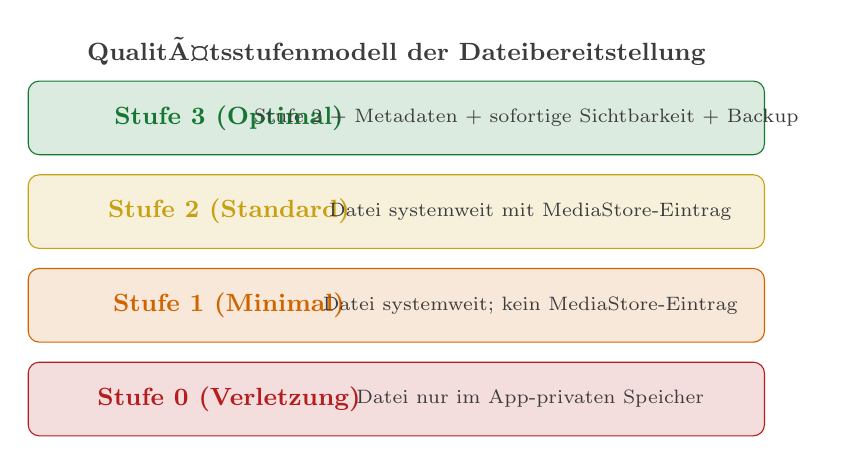
\begin{tikzpicture}[scale=0.85]
\foreach \y/\label/\col/\desc in {
  0/Stufe 0 (Verletzung)/alertred/Datei nur im App-privaten Speicher,
  1.4/Stufe 1 (Minimal)/warnorange/Datei systemweit; kein MediaStore-Eintrag,
  2.8/Stufe 2 (Standard)/accentgold/Datei systemweit mit MediaStore-Eintrag,
  4.2/Stufe 3 (Optimal)/okgreen/Stufe 2 + Metadaten + sofortige Sichtbarkeit + Backup
}{
  \fill[\col!15, draw=\col, rounded corners=4pt] (-5.5, \y-0.55) rectangle (5.5, \y+0.55);
  \node[font=\bfseries\small, color=\col] at (-2.5, \y) {\label};
  \node[font=\scriptsize, color=darkgray, align=left] at (2.0, \y) {\desc};
}
\node[font=\bfseries\small, color=darkgray] at (0, 5.2) {Qualitätsstufenmodell der Dateibereitstellung};
\end{tikzpicture}
\caption{Qualitätsstufen der Dateibereitstellung. Nur Stufe 2 und 3 sind
bereitstellungskonform; Stufe 3 ist die empfohlene Implementierung.}
\label{fig:qualitaet}
\end{figure}

%============================================================
\section{Empfehlungen und Best Practices}
\label{sec:empfehlungen}
%============================================================

\subsection{Für Entwickler}

\begin{enumerate}[label=\textbf{E\arabic*.}]
  \item \textbf{MediaStore als erste Wahl:} Für alle persistenten Mediendateien
    (Bilder, Videos, Audio) immer \texttt{MediaStore} verwenden, nie
    \texttt{getFilesDir()} oder \texttt{getExternalFiles\newline Dir()}.
  \item \textbf{SAF für Dokumente:} Das Storage Access Framework für
    nicht-Mediendateien verwenden, um maximale Benutzerfreiheit zu gewährleisten.
  \item \textbf{DownloadManager für Downloads:} Dateien aus dem Internet über
    \texttt{DownloadMa-\newline nager} herunterladen, der automatisch die systemweite
    Bereitstellung sicherstellt.
  \item \textbf{IS\_PENDING-Muster verwenden:} Beim Schreiben großer Dateien
    das \texttt{IS\_PEN\newline DING}-Flag nutzen, um Integrität sicherzustellen.
  \item \textbf{Sofortige Bereitstellung:} Die Bereitstellung unmittelbar nach
    Abschluss des Erzeugungsprozesses vornehmen, nicht verzögert oder auf
    Benutzerinteraktion wartend.
  \item \textbf{Aussagekräftige Metadaten:} Beim MediaStore-Eintrag vollständige
    Metadaten (Name, MIME-Typ, Datum, Beschreibung) eintragen.
  \item \textbf{Testen mit Integrationstest:} Automatisierte Tests schreiben,
    die die systemweite Verfügbarkeit von erzeugten Dateien prüfen.
\end{enumerate}

\subsection{Für Plattformbetreiber}

\begin{enumerate}[label=\textbf{P\arabic*.}]
  \item \textbf{Linting-Regeln:} Statische Analyse-Werkzeuge um Regeln erweitern,
    die die Verwendung von \texttt{getFilesDir()} für persistente Mediendateien
    als Warnung oder Fehler markieren.
  \item \textbf{App-Store-Reviews:} Systematische Prüfung auf Verletzungen des
    Bereitstellungsprinzips im App-Review-Prozess.
  \item \textbf{Entwicklerdokumentation:} Das Bereitstellungsprinzip explizit in
    Entwicklerdokumentationen als verpflichtend kennzeichnen.
\end{enumerate}

\subsection{Für Benutzer}

\begin{enumerate}[label=\textbf{B\arabic*.}]
  \item \textbf{Apps prüfen:} Überprüfen, ob erzeugte Dateien im Dateimanager
    sichtbar sind. Wenn nicht, ist die App wahrscheinlich bereitstellungswidrig.
  \item \textbf{Feedback geben:} Entwickler über fehlende systemweite
    Bereitstellung informieren (Store-Bewertung, Entwickler-Kontakt).
  \item \textbf{Alternativ-Apps wählen:} Bei systematischer Verletzung des
    Bereitstellungsprinzips auf konforme Alternativen wechseln.
\end{enumerate}

%============================================================
\section{Zusammenfassung}
\label{sec:zusammenfassung}
%============================================================

Die vorliegende Arbeit hat das \emph{Bereitstellungsprinzip} als fundamentalen
Grundsatz mobiler Softwarearchitektur hergeleitet und umfassend analysiert.
Die wesentlichen Erkenntnisse lassen sich wie folgt zusammenfassen:

\noindent\textbf{Kern-Erkenntnisse:}
\begin{enumerate}[leftmargin=*, label=\textbf{\arabic*.}]
  \item \textbf{Das Bereitstellungsprinzip ist unbedingt:} Jede dateiproduzierende
    App \emph{muss} erzeugte Dateien dem systemweiten Speicher zur Verfügung stellen.
    Es gibt keine legitime Ausnahme für persistente Benutzerdaten.
  \item \textbf{Es ist technisch umsetzbar:} Android und iOS bieten vollständige
    API-Unterstützung für korrekte Bereitstellung (MediaStore, SAF, PHPhotoLibrary).
  \item \textbf{Es ist rechtlich geboten:} Datensouveränität, DSGVO und
    Wettbewerbsrecht stützen das Bereitstellungsprinzip.
  \item \textbf{Die Terminologie ist zu präzisieren:} \enquote{Zur Verfügung stellen}
    ist die korrekte Formulierung; sie beschreibt den Normalzustand, nicht
    eine nachträgliche Handlung.
  \item \textbf{Die Konsequenzen sind weitreichend:} Backup, Interoperabilität,
    Barrierefreiheit, Cloud-Sync, Gerätewechsel, Wettbewerb, Rechtskonformität
    --- all diese Bereiche hängen von der Einhaltung des Bereitstellungsprinzips ab.
\end{enumerate}

Das Bereitstellungsprinzip ist keine optionale Qualitätseigenschaft, sondern
ein architektonisches und ethisches Gebot. Mobile Betriebssysteme wurden
konzipiert, um Benutzer zu befähigen — nicht, um Daten in App-Silos zu
fragmentieren. Die Verantwortung für seine Einhaltung liegt bei Entwicklern,
Plattformbetreibern und — durch ihre Marktmacht — bei den Benutzern selbst.

\subsection{Ausblick}
\label{sec:ausblick}

Die in dieser Arbeit dargelegten Grundsätze und Konsequenzen des Bereitstellungsprinzips
sind keineswegs als abgeschlossenes Erkenntnissystem zu verstehen. Die mobile
Computing-Landschaft befindet sich in einem stetigen und teils rasanten Wandel,
der sowohl technische als auch rechtliche und gesellschaftliche Dimensionen umfasst.
Der folgende Ausblick skizziert die wichtigsten Entwicklungstendenzen, die das
Bereitstellungsprinzip in den kommenden Jahren prägen, herausfordern und
weiterentwickeln werden.

\subsubsection{Weiterentwicklung der Plattform-APIs und Betriebssystemarchitekturen}

Die Bereitstellungs-APIs beider großen mobilen Plattformen --- Android und iOS --- befinden
sich in kontinuierlicher Weiterentwicklung. Auf Android-Seite wurde mit der Einführung
von \emph{Scoped Storage} in Android 10 ein grundlegender Paradigmenwechsel vollzogen:
Apps erhalten keinen freien Dateisystemzugriff mehr, sondern operieren über streng
typisierten APIs. Dieser Trend wird sich fortsetzen. Es ist zu erwarten, dass
zukünftige Android-Versionen:
\begin{itemize}[leftmargin=*]
  \item die Granularität des Berechtigungssystems weiter verfeinern, etwa durch
    zeitlich begrenzte oder zweckgebundene Zugriffsberechtigungen auf Mediendateien;
  \item neue \texttt{MediaStore}-Kategorien einführen, die spezialisierte Dateitypen
    (medizinische Daten, Finanzdokumente, Bildungsmaterialien) semantisch erfassen;
  \item die \emph{Health\,Connect}-Plattform als Modell für zukünftige, datentypspezifische
    Bereitstellungs-APIs etablieren --- ähnlich wie HealthKit auf iOS einen
    standardisierten, sicheren Datenaustausch für Gesundheitsdaten ermöglicht;
  \item einen erweiterten \emph{Photo Picker} bereitstellen, der Anwendungen den Zugriff
    auf Mediendateien ohne vollständige Lese-Berechtigungen ermöglicht und damit das
    Bereitstellungsprinzip schreibend von App-Seite konsequent einfordert.
\end{itemize}

Auf iOS-Seite ist eine sukzessive Öffnung des Dateisystems zu beobachten, die mit iOS 11
durch die Files-App und das \texttt{UIDocumentBrowserViewController}-Framework eingeleitet
wurde. Zukünftige iOS-Versionen werden voraussichtlich die Inter-App-Kommunikation auf
Dateiebene weiter erleichtern, das \emph{Shared with You}-Framework ausbauen und die
Abhängigkeit von proprietären iCloud-Strukturen reduzieren, indem offene Dateiformate und
standardisierte Metadaten bevorzugt werden.

Ein besonders bedeutsamer Trend ist die zunehmende Konvergenz zwischen Desktop- und
mobilen Betriebssystemen. Apples \emph{Catalyst}-Technologie und Microsofts Integration
von Android-Apps unter Windows (Windows Subsystem for Android) deuten darauf hin, dass
die scharfe Grenze zwischen mobilen und Desktop-Dateisystemparadigmen langfristig
verschwimmen könnte. Das Bereitstellungsprinzip wird dabei als Brückenkonzept fungieren
müssen, das mobile Bereitstellungsmechanismen mit klassischen Desktop-Dateisystemzugriffen
harmonisiert.

\subsubsection{Das Origin Private File System und webbasierte Speicherparadigmen}

Die Entstehung des \emph{Origin Private File System} (OPFS) im Rahmen des
\emph{File System Access API}-Standards des W3C stellt eine fundamentale Herausforderung
für das Bereitstellungsprinzip im Web-Kontext dar. OPFS bietet Progressive Web Apps einen
performanten, privaten Dateispeicher --- analog zum App-privaten Speicher nativer Apps.
Gleichzeitig haben Progressive Web Apps über die \texttt{showSaveFilePicker()}-API die
Möglichkeit, Dateien in den systemweiten Speicher zu schreiben.

Die Frage, welche dieser APIs für welchen Dateityp zu verwenden ist, spiegelt unmittelbar
das Bereitstellungsprinzip wider: Temporäre Arbeitsdaten gehören in OPFS; persistente
Benutzerdateien müssen über \texttt{showSaveFilePicker()} dem System zugänglich gemacht
werden. Zukünftige Forschung sollte untersuchen, ob und wie das Bereitstellungsprinzip
formal auf das Web-Ökosystem übertragen werden kann, insbesondere in Anbetracht der
unterschiedlichen Sicherheitsmodelle zwischen Same-Origin-Policy und dem
Android-Sandboxing-Ansatz.

\subsubsection{Regulatorische und rechtliche Entwicklungen}

Das rechtliche Umfeld für mobile Betriebssysteme und App-Öko\-sys\-te\-me befindet sich
in einem historisch einzigartigen Wandel. Mehrere regulatorische Entwicklungen werden
das Bereitstellungsprinzip direkt oder indirekt stärken.

\paragraph{Digital Markets Act (DMA).}
Der im November 2022 in Kraft getretene \emph{Digital Markets Act} der Europäischen Union
verpflichtet sogenannte \emph{Gatekeeper} --- zu denen Apple und Google mit ihren
App-Ökosystemen zählen --- zu weitreichender Interoperabilität und Datenportabilität.
Art.\,6 Abs.\,9 DMA verlangt insbesondere, dass Gatekeeper Nutzern den Zugang zu ihren
generierten Daten ermöglichen. Dies deckt sich exakt mit dem Bereitstellungsprinzip:
Daten, die auf einem Gerät erzeugt wurden, müssen dem Nutzer zugänglich sein. Zukünftige
DMA-Durchsetzungsverfahren könnten explizit auf das Bereitstellungsprinzip als technischen
Standard verweisen und damit seine Verbindlichkeit auf Plattformebene durchsetzen.

\paragraph{Data Act.}
Der im März 2024 in Kraft getretene \emph{Data Act} (Verordnung (EU) 2023/2854) schafft
horizontale Regeln für den Datenzugang und die Datennutzung in der gesamten EU-Wirtschaft.
Für mobile Apps, die Nutzerdaten erzeugen, ergibt sich die Verpflichtung, diese Daten in
interoperablen Formaten bereitzustellen. Das Bereitstellungsprinzip wird durch den Data Act
eine explizite rechtliche Grundlage erhalten, die über die bisher aus der DSGVO mittelbar
ableitbare Datenzugangsregelung hinausgeht.

\paragraph{AI Act und dateibasierte KI-Trainingsdaten.}
Die \emph{Verordnung über Künstliche Intelligenz} (AI Act, Verordnung (EU) 2024/1689)
führt neue Anforderungen an die Nachvollziehbarkeit von KI-Trainingsdaten ein. Wenn
mobile Apps auf geräteerzeugten Dateien KI-Modelle trainieren oder diese Daten für
systemische KI-Anwendungen verwenden, entsteht ein Spannungsfeld zwischen dem
Bereitstellungsprinzip (Daten sollen systemweit zugänglich sein) und dem Schutz vor
unerwünschter KI-Nutzung dieser Daten. Zukünftige Forschung muss untersuchen, wie das
Bereitstellungsprinzip in KI-regulierten Umgebungen zu kalibrieren ist.

\paragraph{Internationaler Rechtsrahmen.}
Außerhalb der EU entstehen vergleichbare Regelungstendenzen: Der \emph{American Data
Privacy and Protection Act} (ADPPA), das \emph{California Consumer Privacy Act} (CCPA)
und Regelungen in Asien (Japans APPI, Indiens DPDP Act) konvergieren zunehmend auf
gemeinsame Prinzipien der Datensouveränität, die das hier beschriebene Bereitstellungs\-prinzip
international stützen.

\subsubsection{Technologische Trends: Cloud-native Storage und Hybridarchitekturen}

Die zunehmende Durchdringung mobiler Geräte mit permanenter Internetverbindung führt
zu neuen Speicherparadigmen, die das Bereitstellungsprinzip in seiner klassischen,
lokal orientierten Form herausfordern.

\paragraph{Cloud-as-Primary-Storage.}
Dienste wie Google Drive, iCloud Drive und OneDrive werden zunehmend nicht mehr als
nachgelagerte Synchronisationsschicht, sondern als primärer Speicherort für erzeugte
Dateien betrachtet. Das Bereitstellungsprinzip muss in diesem Kontext auf cloud-basierte
Speicherziele ausgedehnt werden: Eine dateiproduzierende App, die Dateien direkt in der
Cloud speichert, muss sicherstellen, dass diese Dateien über standardisierte
Schnittstellen (WebDAV, CMIS, proprietäre Cloud-APIs) für den Benutzer zugänglich sind.

\paragraph{FUSE und virtuelle Dateisysteme.}
\emph{Filesystem in Userspace} (FUSE) ermöglicht die transparente Integration von
Remotspeichern in lokale Dateistrukturen. Zukünftige mobile Betriebssysteme könnten
FUSE-artige Mechanismen einsetzen, um cloud-basierte und lokale Speicher unter einer
einheitlichen Dateisystemabstraktion zusammenzuführen. Das Bereitstellungsprinzip würde
davon profitieren: Eine Datei, die in einem virtuellen Dateisystem abgelegt ist, wäre
automatisch systemweit verfügbar, unabhängig von ihrem physischen Speicherort.

\paragraph{Peer-to-Peer-Dateisysteme.}
Dezentrale Dateisysteme wie \emph{IPFS} (InterPlanetary File System) beginnen, in mobilen
Anwendungsszenarien Relevanz zu erlangen. In solchen Systemen erfolgt die Bereitstellung
nicht mehr über einen zentralen Systemdienst (MediaStore, Files-App), sondern über ein
Netzwerkprotokoll. Das Bereitstellungsprinzip muss in diesem Fall auf die Frage erweitert
werden, ob und wie eine Datei für den \emph{Eigentümer} auffindbar und zugreifbar bleibt,
auch wenn sie dezentral gespeichert ist.

\subsubsection{Künstliche Intelligenz und semantische Dateiverwaltung}

Vielleicht die tiefgreifendste Transformation des mobilen Dateisystems steht durch den
Einsatz von KI-Methoden bevor. Aktuelle Entwicklungen lassen folgende Trends erkennen:

\paragraph{Automatische Dateikategorisierung.}
KI-gestützte Systeme (wie Googles \emph{Gemini}-Integration in Android oder Apples
\emph{Intelligence}-Funktionen) sind zunehmend in der Lage, Dateiinhalte semantisch zu
verstehen und automatisch zu kategorisieren. Zukünftig könnten mobile Betriebssysteme
Dateien automatisch dem richtigen systemweiten Bereitstellungsziel zuordnen: Ein
KI-Modell erkennt, dass eine erzeugte Datei ein Bild ist, und legt sie automatisch im
korrekten \texttt{MediaStore}-Bucket ab, ohne dass die App explizit eine \texttt{insert()}-Operation
aufrufen muss. Dies würde das technische Risiko von Bereitstellungsverletzungen aus
Implementierungsfehlern erheblich reduzieren.

\paragraph{On-Device-AI und datenschutzwahrende Verarbeitung.}
Die Verlagerung von KI-Verarbeitung auf das Gerät selbst (On-Device-AI) erzeugt neue
Arten dateiproduzierender Prozesse: KI-generierte Bilder, zusammengefasste Dokumente,
transkribierte Audiodateien. Das Bereitstellungsprinzip gilt für diese Ausgaben
uneingeschränkt --- auch KI-erzeugte Inhalte müssen systemweit zugänglich gemacht werden,
wenn der Benutzer sie als persistente Ergebnisse betrachtet.

\paragraph{Semantische Metadatenanreicherung.}
Zukünftige Bereitstellungssysteme werden über reine Dateipfade hinausgehen und Dateien
mit semantischen Metadaten anreichern. Der \texttt{MediaStore} könnte um Felder für
KI-erzeugte Beschreibungen, erkannte Objekte oder inhaltliche Zusammenfassungen erweitert
werden. Das Bereitstellungsprinzip müsste in diesem Fall nicht nur die \emph{physische}
Verfügbarkeit einer Datei fordern, sondern auch ihre \emph{semantische} Auffindbarkeit
durch systemweite Suchfunktionen.

\subsubsection{Sicherheit und datenschutzfreundliche Bereitstellungsarchitekturen}

Das Spannungsverhältnis zwischen systemweiter Bereitstellung und Datenschutz wird in
Zukunft durch neue technische Architekturen aufgelöst werden müssen.

\paragraph{Vertrauliche Bereitstellung.}
Eine vielversprechende Forschungsrichtung ist die \emph{vertrauliche Bereitstellung}:
Dateien werden systemweit bereitgestellt, jedoch in einer Weise verschlüsselt, die nur
authorisierten Apps und Benutzern den Inhaltszugriff ermöglicht. Technologien wie
\emph{Trusted Execution Environments} (TEE) auf ARM-Prozessoren (TrustZone) könnten
als Basis für schlüsselverwaltende Bereitstellungsinfrastruktur dienen. In diesem Modell
ist eine Datei \emph{auffindbar} (Bereitstellungsprinzip erfüllt) und gleichzeitig
\emph{inhaltlich geschützt} (Datenschutz gewahrt).

\paragraph{Attributbasierte Zugangskontrolle.}
Klassische Zugangskontrolle basiert auf Identitäten (welche App darf zugreifen?).
Zukünftige Systeme könnten \emph{attributbasierte Zugangskontrolle} (ABAC) einsetzen:
Eine Datei ist systemweit bereitgestellt, aber Zugriff wird nur Anwendungen gewährt,
die bestimmte Attribute aufweisen (z.\,B. \enquote{ist als medizinische App zertifiziert}
oder \enquote{hat explizite Nutzerfreigabe für diesen Dateityp}). Dies würde das
Bereitstellungsprinzip mit feingranularem Datenschutz verbinden.

\paragraph{Datensparsamkeit und typenspezifische Bereitstellung.}
Im Lichte von Art.\,5 Abs.\,1 lit.\,c DSGVO (Datensparsamkeit) entsteht die Frage, ob
das Bereitstellungsprinzip zu einer systemweiten Nachverfolgbarkeit führen kann, die dem
Datensparsamkeitsprinzip widerspricht. Konzeptuell ist zu betonen: Das Bereitstellungsprinzip
fordert \emph{Zugänglichkeit für den Benutzer}, nicht \emph{Sichtbarkeit für Dritte}.
Zukünftige Implementierungen müssen diese Unterscheidung technisch präziser abbilden.

\subsubsection{IoT, Edge Computing und erweiterte Geräteklassen}

Die Grenzen des \enquote{mobilen Geräts} verschwimmen zunehmend. Smartwatches,
AR/VR-Brillen, Connected Cars und smarte Haushaltsgeräte werden zu dateiproduzierenden
Systemen, für die das Bereitstellungsprinzip Anwendung finden muss.

\paragraph{Wearables und Gesundheitsdaten.}
Smartwatch- und Fitness-Tracker-Apps erzeugen kontinuierlich Dateien (Schlafprotokolle,
EKG-Aufzeichnungen, Bewegungsdaten). Die zugehörigen mobilen Apps müssen diese Daten
über APIs wie Apple HealthKit (iOS) oder Android Health Connect systemweit bereitstellen.
Die besondere Sensibilität dieser Daten (Art.\,9 DSGVO: besondere Kategorien
personenbezogener Daten) erfordert dabei ein differenzierteres Bereitstellungsmodell,
das Zugänglichkeit und Schutz ausbalanciert.

\paragraph{AR/VR-Geräte und räumliche Daten.}
Augmented-Reality- und Virtual-Reality-Headsets (Apple Vision Pro, Meta Quest) erzeugen
neuartige Dateiformate: räumliche Scans, 3D-Objekte, immersive Videoinhalte. Es ist zu
erwarten, dass zukünftige \texttt{MediaStore}-Kategorien diese Dateitypen aufnehmen
werden. Das Bereitstellungsprinzip postuliert: Auch 3D-Inhalte, die auf einem
AR/VR-Gerät erzeugt werden, müssen über standardisierte APIs dem System zur Verfügung
gestellt werden.

\paragraph{Vernetzte Fahrzeuge und mobile Arbeitsumgebungen.}
In moderne Kraftfahrzeuge integrierte Betriebssysteme (Android Automotive,
CarPlay-unterstützte Systeme) bilden erweiterte mobile Plattformen. Dashcam-Aufnahmen,
Navigationshistorien und fahrzeugintern erzeugte Dokumente fallen unter das
Bereitstellungsprinzip. Zukünftige Fahrzeugbetriebssysteme werden einen eigenen
Medienspeicher entwickeln müssen, der mit mobilen Gerätearchiven synchronisiert
werden kann.

\subsubsection{Standardisierung und internationale Interoperabilität}

Ein wesentliches Desiderat der zukünftigen Forschung und Normierungsarbeit ist die
plattformübergreifende Standardisierung des Bereitstellungsprinzips.

\paragraph{W3C-Standardisierung.}
Die \emph{File System Access API} des W3C ist ein erster Schritt zur Standardisierung
webbasierter Dateibereitstellung. Zukünftige W3C-Standards sollten explizit das
Bereitstellungsprinzip kodieren und klare Anforderungen an das Schreiben persistenter
Nutzerdaten in zugängliche Speicherbereiche formulieren. Das \emph{Storage Foundation API}
ist ein vielversprechender Anknüpfungspunkt für diese Standardisierungsarbeit.

\paragraph{ISO/IEC-Normierung.}
Im Bereich der mobilen Anwendungssicherheit existieren Normen wie ISO/IEC\,27034
(Application Security). Eine Erweiterung dieser Normen um explizite Anforderungen an
die Dateibereitstellung würde das Bereitstellungsprinzip in international anerkannte
Qualitätsstandards integrieren.

\paragraph{Plattformübergreifende Interoperabilität.}
Das größte offene Problem ist die Interoperabilität zwischen Android und iOS. Eine
auf iOS erstellte Datei kann nicht automatisch über den Android-MediaStore zugänglich
gemacht werden und umgekehrt. Cloud-Synchronisationsdienste lösen dieses Problem
partiell, setzen aber proprietäre Infrastruktur voraus. Eine zukünftige
\emph{Mobile File Provisioning Interoperability Specification} --- vergleichbar mit
dem \emph{WebDAV}-Standard für Netzwerkdateisysteme --- könnte plattformübergreifende
Bereitstellung ohne Cloud-Abhängigkeit realisieren.

\subsubsection{Offene Forschungsfragen}

Die vorliegende Arbeit wirft eine Reihe von Forschungsfragen auf, die einer
systematischen wissenschaftlichen Bearbeitung bedürfen:

\begin{enumerate}[label=\textbf{F\arabic*.}, leftmargin=*]
  \item \textbf{Formale Verifikation:} Lässt sich das Bereitstellungsprinzip in formale
    App-Verifi\-kationswerkzeuge integrieren? Können statische Analysatoren (z.\,B. auf
    Basis von \emph{Datalog}-Regeln oder Typtheorie) Verletzungen des
    Bereitstellungsprinzips zur Compile-Zeit erkennen?
  \item \textbf{Automatisches Refactoring:} Können KI-gestützte Code-Transformatoren
    (z.\,B.\ GitHub Copilot oder ähnliche Systeme) Implementierungen, die gegen das
    Bereitstellungsprinzip verstoßen, automatisch identifizieren und korrekte Alternativen
    vorschlagen?
  \item \textbf{Empirische Prävalenz:} Wie verbreitet sind Verletzungen des
    Bereitstellungsprinzips in der realen App-Landschaft? Eine systematische Analyse
    über den Google Play Store und den Apple App Store --- basierend auf statischer
    Analyse und Laufzeittests --- könnte empirische Daten zu dieser Frage liefern.
  \item \textbf{Benutzerpräferenzen:} Welche Präferenzen haben Benutzer bezüglich der
    Zugänglichkeit ihrer erzeugten Dateien? Empirische Usability-Studien könnten das
    Bereitstellungsprinzip durch nutzerzentrierte Evidenz stützen oder differenzieren.
  \item \textbf{Performanz-Implikationen:} Hat die systemweite Bereitstellung von Dateien
    messbare Auswirkungen auf die App-Performanz (Latenz beim Schreiben,
    Energie\-verbrauch durch MediaStore-Operationen)? Benchmarking-Studien könnten die
    praktischen Kosten der korrekten Implementierung quantifizieren.
  \item \textbf{Quantitativer Datenverlust:} Wie groß ist der tatsächliche Datenverlust,
    der durch Verletzungen des Bereitstellungsprinzips entsteht? Eine Befragungsstudie
    mit mobilen Nutzern, die Datenverluste nach App-Deinstallationen erlebt haben, könnte
    die gesellschaftlichen Kosten dieser Verletzungen sichtbar machen.
  \item \textbf{Semantisches Bereitstellungsmodell:} Ist ein erweitertes
    Bereitstellungsmodell denkbar, das nicht nur Dateien, sondern auch strukturierte Daten
    (Datenbanken, App-Zustände, Konfigurationen) dem Bereitstellungsprinzip unterwirft?
    Diese Erweiterung würde das Bereitstellungsprinzip zu einem umfassenden
    \emph{Datensouveränitätsprinzip} für mobile Geräte verallgemeinern.
\end{enumerate}

\subsubsection{Langfristige Vision: Das benutzerzentristische Dateisystem}

Auf einer übergeordneten Ebene zeigt die vorliegende Analyse, dass das
Bereitstellungsprinzip Teil einer größeren Vision für mobile Betriebssysteme ist:
das \emph{benutzerzentrische Dateisystem}, in dem der Benutzer --- nicht die App ---
als Eigentümer und primärer Verwalter aller erzeugten Daten fungiert.

Diese Vision impliziert einen strukturellen Wandel: Statt dass Apps entscheiden,
\emph{wo} und \emph{wie} Dateien gespeichert werden, übernimmt das Betriebssystem
die Verantwortung für eine optimale Bereitstellung, basierend auf Dateityp,
Nutzungspräferenzen und rechtlichen Anforderungen. Apps werden zu reinen Produzenten;
das Betriebssystem wird zum intelligenten Verteiler und Verwalter.

Technologische Bausteine für diese Vision sind bereits erkennbar: Androids
\texttt{MediaStore} mit seinen typisierten Buckets, Apples \texttt{PHPhotoLibrary}
mit ihrer nicht-destruktiven Bearbeitungsphilosophie, Googles
\emph{Personal Data Store}-Konzepte --- all diese Entwicklungen deuten in dieselbe
Richtung. Das Bereitstellungsprinzip ist damit nicht nur ein technischer Grundsatz
der gegenwärtigen mobilen Softwareentwicklung, sondern auch ein Wegweiser für die
Architektur zukünftiger mobiler Betriebssysteme.

Die konsequente Anwendung und Weiterentwicklung des Bereitstellungsprinzips wird
langfristig dazu beitragen, das Vertrauen der Nutzer in mobile Plattformen zu stärken,
digitale Souveränität zu fördern und eine fairere, interoperablere digitale Infrastruktur
zu schaffen --- eine Infrastruktur, in der Daten dem dienen, der sie erzeugt hat:
dem Benutzer selbst.

%============================================================
\begin{thebibliography}{99}
\addcontentsline{toc}{section}{Literaturverzeichnis}
%============================================================

\bibitem{android-scoped-storage}
Google LLC.
\newblock \emph{Scoped Storage changes in Android 10}.
\newblock Android Developers Documentation, 2019.
\newblock \url{https://developer.android.com/about/versions/10/privacy/changes#scoped-storage}

\bibitem{android-mediastore}
Google LLC.
\newblock \emph{MediaStore API Reference}.
\newblock Android Developers Documentation, 2024.
\newblock \url{https://developer.android.com/reference/android/provider/MediaStore}

\bibitem{android-storage-overview}
Google LLC.
\newblock \emph{Data and file storage overview}.
\newblock Android Developers Documentation, 2024.
\newblock \url{https://developer.android.com/training/data-storage}

\bibitem{android-saf}
Google LLC.
\newblock \emph{Open files using storage access framework}.
\newblock Android Developers Documentation, 2024.
\newblock \url{https://developer.android.com/guide/topics/providers/document-provider}

\bibitem{android-fileprovider}
Google LLC.
\newblock \emph{FileProvider --- Setting Up File Sharing}.
\newblock Android Developers Documentation, 2024.
\newblock \url{https://developer.android.com/reference/androidx/core/content/FileProvider}

\bibitem{android-downloadmanager}
Google LLC.
\newblock \emph{DownloadManager API Reference}.
\newblock Android Developers Documentation, 2024.
\newblock \url{https://developer.android.com/reference/android/app/DownloadManager}

\bibitem{android-permissions}
Google LLC.
\newblock \emph{Request app permissions --- Android Developers}.
\newblock Android Developers Documentation, 2024.
\newblock \url{https://developer.android.com/training/permissions/requesting}

\bibitem{android-mediascanner}
Google LLC.
\newblock \emph{MediaScannerConnection --- Android Developers}.
\newblock Android Developers Documentation, 2024.
\newblock \url{https://developer.android.com/reference/android/media/MediaScannerConnection}

\bibitem{android-autobackup}
Google LLC.
\newblock \emph{Back up user data with Auto Backup}.
\newblock Android Developers Documentation, 2024.
\newblock \url{https://developer.android.com/identity/data/autobackup}

\bibitem{ios-phphotolibrary}
Apple Inc.
\newblock \emph{PHPhotoLibrary --- PhotoKit Framework Reference}.
\newblock Apple Developer Documentation, 2024.
\newblock \url{https://developer.apple.com/documentation/photokit/phphotolibrary}

\bibitem{ios-files-framework}
Apple Inc.
\newblock \emph{File System Programming Guide for iOS}.
\newblock Apple Developer Documentation, 2023.
\newblock \url{https://developer.apple.com/library/archive/documentation/FileManagement/Conceptual/FileSystemProgrammingGuide/Introduction/Introduction.html}

\bibitem{ios-document-browser}
Apple Inc.
\newblock \emph{UIDocumentBrowserViewController --- Providing Access to Directories}.
\newblock Apple Developer Documentation, 2024.
\newblock \url{https://developer.apple.com/documentation/uikit/uidocumentbrowserviewcontroller}

\bibitem{ios-icloud-backup}
Apple Inc.
\newblock \emph{iCloud Storage and Backup Overview}.
\newblock Apple Developer Documentation, 2024.
\newblock \url{https://developer.apple.com/icloud/documentation/}

\bibitem{dsgvo-text}
Europäisches Parlament und Rat der Europäischen Union.
\newblock \emph{Verordnung (EU) 2016/679 des Europäischen Parlaments und des Rates
  (Datenschutz-Grundverordnung)}.
\newblock Amtsblatt der Europäischen Union, L~119, S.~1--88, 4.~Mai 2016.

\bibitem{dma-text}
Europäisches Parlament und Rat der Europäischen Union.
\newblock \emph{Verordnung (EU) 2022/1925 über bestreitbare und faire Märkte im
  digitalen Sektor (Digital Markets Act)}.
\newblock Amtsblatt der Europäischen Union, L~265, S.~1--66, 12.~Oktober 2022.

\bibitem{data-act-text}
Europäisches Parlament und Rat der Europäischen Union.
\newblock \emph{Verordnung (EU) 2023/2854 über harmonisierte Vorschriften für einen
  fairen Datenzugang und eine faire Datennutzung (Data Act)}.
\newblock Amtsblatt der Europäischen Union, L~2023/2854, 13.~Dezember 2023.

\bibitem{ai-act-text}
Europäisches Parlament und Rat der Europäischen Union.
\newblock \emph{Verordnung (EU) 2024/1689 zur Festlegung harmonisierter Vorschriften
  für künstliche Intelligenz (Gesetz über künstliche Intelligenz)}.
\newblock Amtsblatt der Europäischen Union, L~2024/1689, 12.~Juli 2024.

\bibitem{sandboxing-security}
Enck, W., Ongtang, M., und McDaniel, P.
\newblock \emph{On Lightweight Mobile Phone Application Certification}.
\newblock In: \emph{Proceedings of the 16th ACM Conference on Computer and
  Communications Security (CCS~'09)}, S.~235--245. ACM, 2009.

\bibitem{android-security-overview}
Smalley, S., und Craig, R.
\newblock \emph{Security Enhanced (SE) Android: Bringing Flexible MAC to Android}.
\newblock In: \emph{Proceedings of the 20th Annual Network \& Distributed System
  Security Symposium (NDSS~2013)}. Internet Society, 2013.

\bibitem{mobile-privacy-survey}
Felt, A.\,P., Ha, E., Egelman, S., Haney, A., Chin, E., und Wagner, D.
\newblock \emph{Android Permissions: User Attention, Comprehension, and Behavior}.
\newblock In: \emph{Proceedings of the 8th Symposium on Usable Privacy and Security
  (SOUPS~2012)}. ACM, 2012.

\bibitem{data-sovereignty}
Zuboff, S.
\newblock \emph{The Age of Surveillance Capitalism: The Fight for a Human Future
  at the New Frontier of Power}.
\newblock PublicAffairs, New York, 2019.

\bibitem{vendor-lockin}
Shapiro, C., und Varian, H.\,R.
\newblock \emph{Information Rules: A Strategic Guide to the Network Economy}.
\newblock Harvard Business School Press, Boston, 1999.

\bibitem{w3c-file-system-access}
W3C WHATWG.
\newblock \emph{File System Standard}.
\newblock Living Standard, 2024.
\newblock \url{https://fs.spec.whatwg.org/}

\bibitem{ipfs-whitepaper}
Benet, J.
\newblock \emph{IPFS --- Content Addressed, Versioned, P2P File System}.
\newblock arXiv:1407.3561, 2014.
\newblock \url{https://arxiv.org/abs/1407.3561}

\bibitem{tee-trustzone}
Pinto, S., und Santos, N.
\newblock \emph{Demystifying Arm TrustZone: A Comprehensive Survey}.
\newblock \emph{ACM Computing Surveys}, 51(6):130:1--130:36, 2019.

\bibitem{abac-model}
Hu, V.\,C., Ferraiolo, D., Kuhn, R., Friedman, A.\,R., Lang, A.\,J.,
  Cogdell, M.\,M., Schnitzer, A., Sandlin, K., Miller, R., und Scarfone, K.
\newblock \emph{Guide to Attribute Based Access Control (ABAC) Definition and
  Considerations}.
\newblock NIST Special Publication 800-162. NIST, 2014.

\bibitem{on-device-ai}
Howard, A., Sandler, M., Chu, G., Chen, L.-C., Chen, B., Tan, M., Wang, W.,
  Zhu, Y., Pang, R., Vasudevan, V., Le, Q.\,V., und Adam, H.
\newblock \emph{Searching for MobileNetV3}.
\newblock In: \emph{Proceedings of the IEEE/CVF International Conference on
  Computer Vision (ICCV~2019)}, S.~1314--1324. IEEE, 2019.

\bibitem{android-health-connect}
Google LLC.
\newblock \emph{Health Connect --- Android Developers}.
\newblock Android Developers Documentation, 2024.
\newblock \url{https://developer.android.com/health-and-fitness/guides/health-connect}

\bibitem{digital-markets-act-enforcement}
Europäische Kommission.
\newblock \emph{Digital Markets Act: Erster Bewertungsbericht zu den Gatekeeper-Verpflichtungen}.
\newblock Europäische Kommission, Brüssel, 2024.
\newblock \url{https://commission.europa.eu/strategy-and-policy/priorities-2019-2024/europe-fit-digital-age/digital-markets-act-ensuring-fair-and-contestable-digital-markets_de}

\bibitem{mobile-os-architecture}
Tanenbaum, A.\,S., und Bos, H.
\newblock \emph{Modern Operating Systems}, 4.~Auflage.
\newblock Pearson, Upper Saddle River, NJ, 2015.

\bibitem{android-app-components}
Google LLC.
\newblock \emph{Application Fundamentals --- Android Developers}.
\newblock Android Developers Documentation, 2024.
\newblock \url{https://developer.android.com/guide/components/fundamentals}

\bibitem{content-provider}
Google LLC.
\newblock \emph{Content providers --- Android Developers}.
\newblock Android Developers Documentation, 2024.
\newblock \url{https://developer.android.com/guide/topics/providers/content-providers}

\bibitem{accessibility-guidelines}
World Wide Web Consortium (W3C).
\newblock \emph{Web Content Accessibility Guidelines (WCAG) 2.2}.
\newblock W3C Recommendation, 5.~Oktober 2023.
\newblock \url{https://www.w3.org/TR/WCAG22/}

\end{thebibliography}

\end{document}

